\documentclass[12pt]{beamer}
\usetheme{Goettingen}
\usecolortheme{dove}
\setbeamercovered{transparent}
\setbeamerfont{frametitle}{size=\normalsize} 
\setbeamertemplate{footline}[frame number]
\setbeamertemplate{itemize items}[circle]

\usepackage{graphicx} % images
\usepackage[style=authoryear, maxcitenames=1]{biblatex} % citations + references
\addbibresource{latex/zotero.bib} % zotero bibliography

\usepackage[dvipsnames]{xcolor} % textcolor

\title{Estimating Timescale Maps with fMRI}
\author[]{Gabriel Riegner}
\date{May 2024}

\begin{document}

% slide %
\begin{frame}{Estimating Timescale Maps with Functional MRI}
\small
\begin{columns}
\column{0.5\textwidth}
\tableofcontents[hideallsubsections]
\column{0.5\textwidth}
\visible{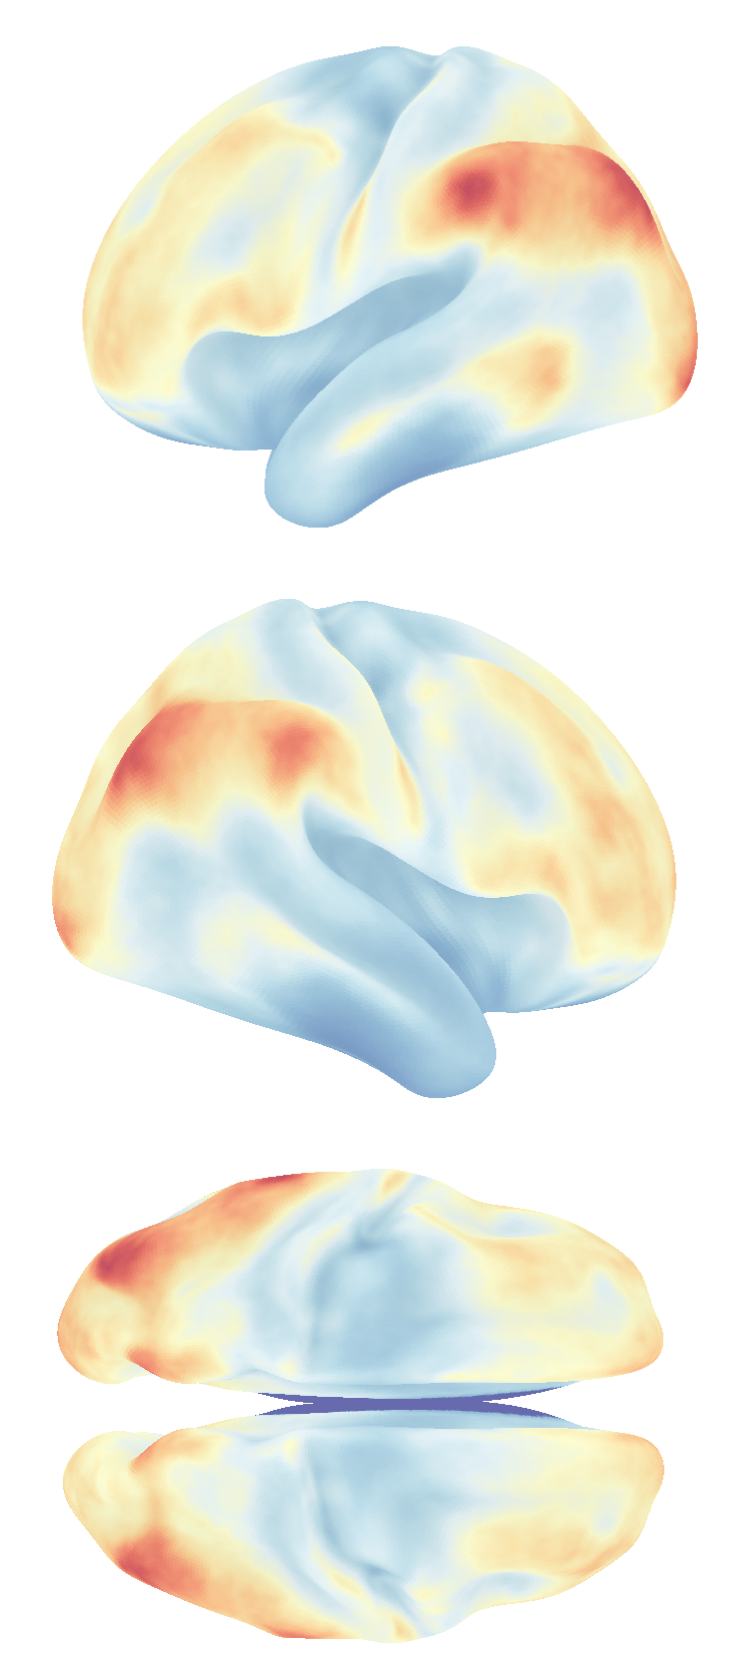
\includegraphics[width=0.5\textwidth]{latex/slides/hcp7T.png}}
\end{columns}
\end{frame}


\section{Motivations}

% slide % 
\subsection{Scientific}
\begin{frame}{Scientific Motivation}
\footnotesize

Neural timeseries often exhibit time-lagged correlation that is characterized by autocorrelations that decay exponentially.\\
\vspace{.5cm}
The timescale parameters ($\tau$) controls the decay rate.
\visible{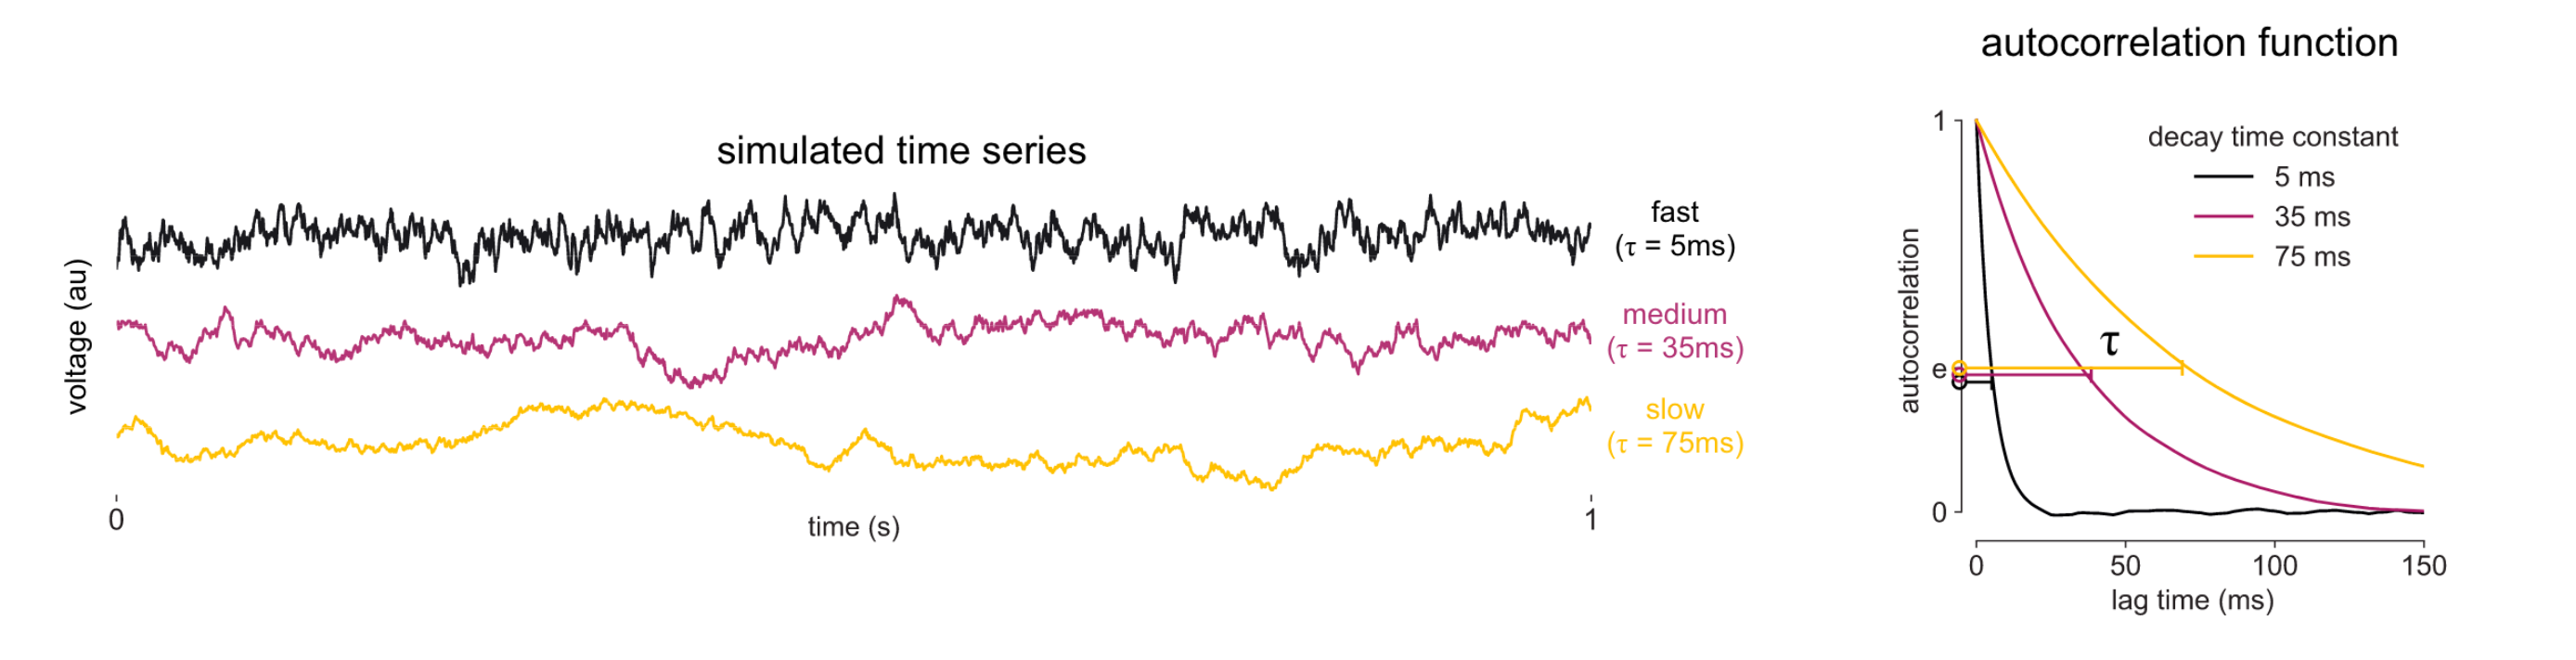
\includegraphics[width=0.95\textwidth]{latex/slides/gao-et-al.png}}
(\cite{gao_neuronal_2020})
\end{frame}

% slide %
\begin{frame}{Timescale Organization}
\footnotesize
Timescales follow a hierarchy from sensory to associative regions of cortex (\cite{murray_hierarchy_2014}).
\visible{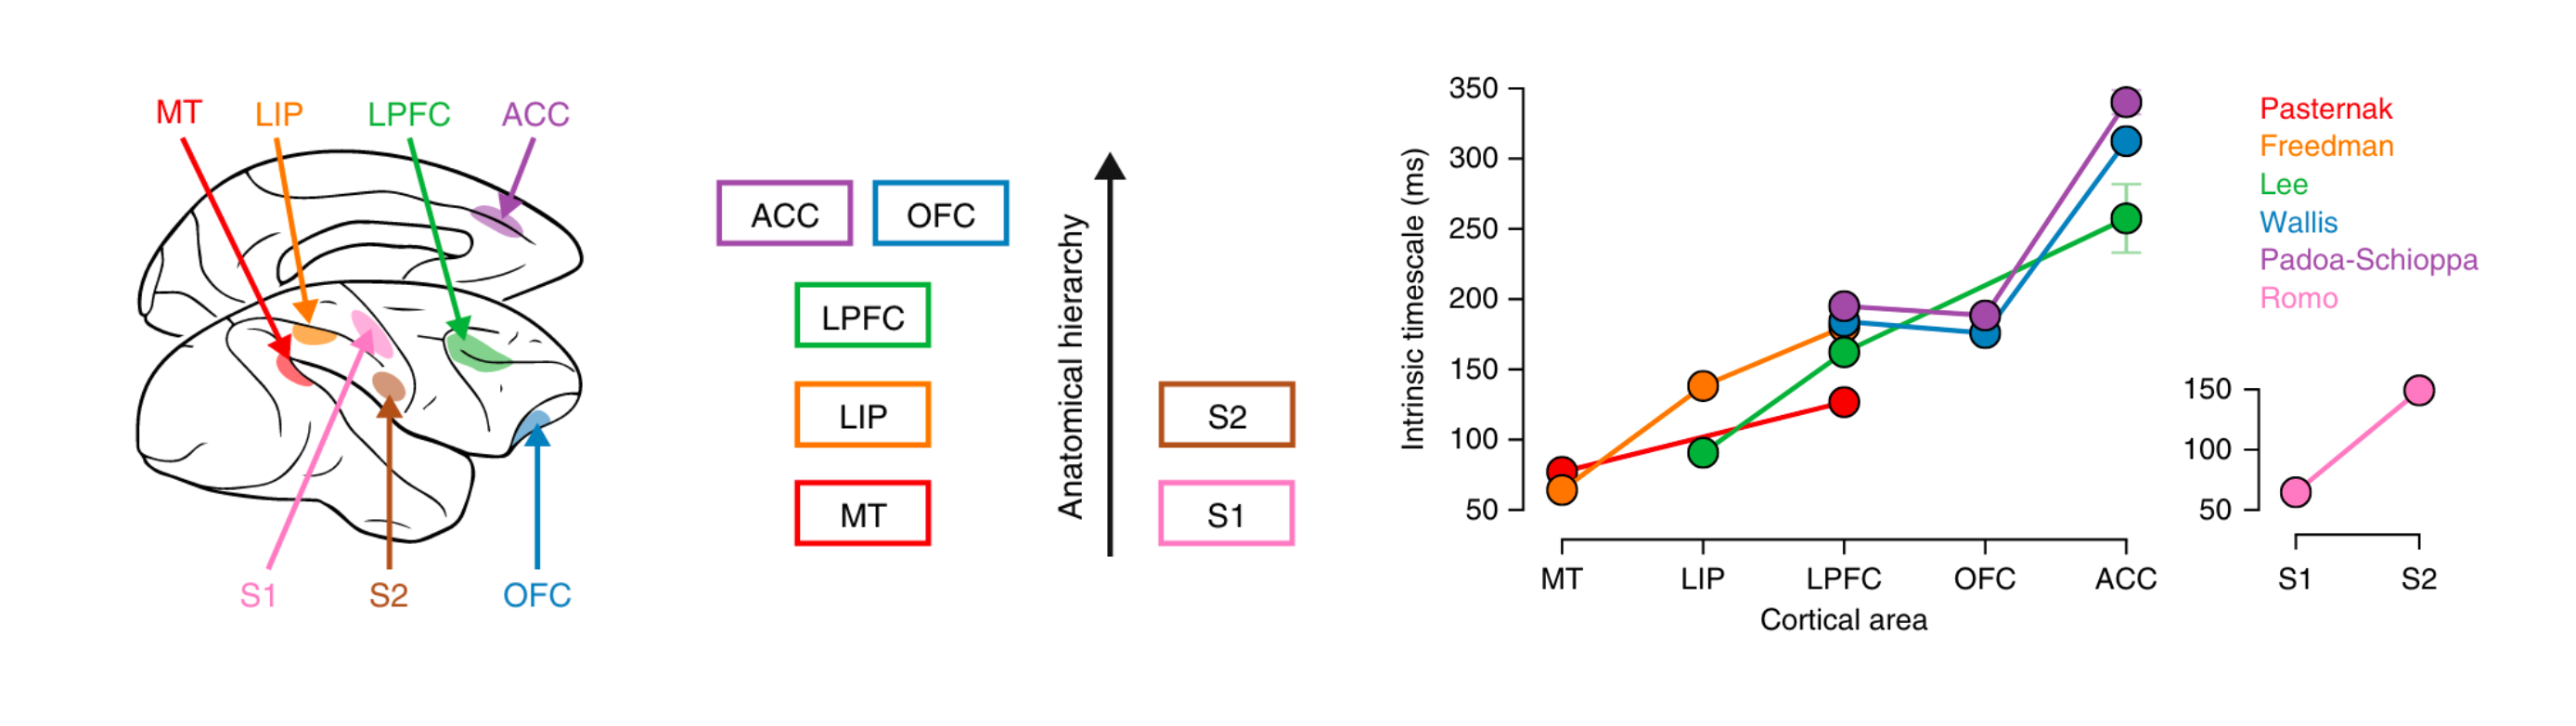
\includegraphics[width=0.95\textwidth]{latex/slides/murray-et-al.png}}

This pattern repeats itself in subcortical regions (\cite{raut_hierarchical_2020, muller_core_2020, nougaret_intrinsic_2021}).
\visible{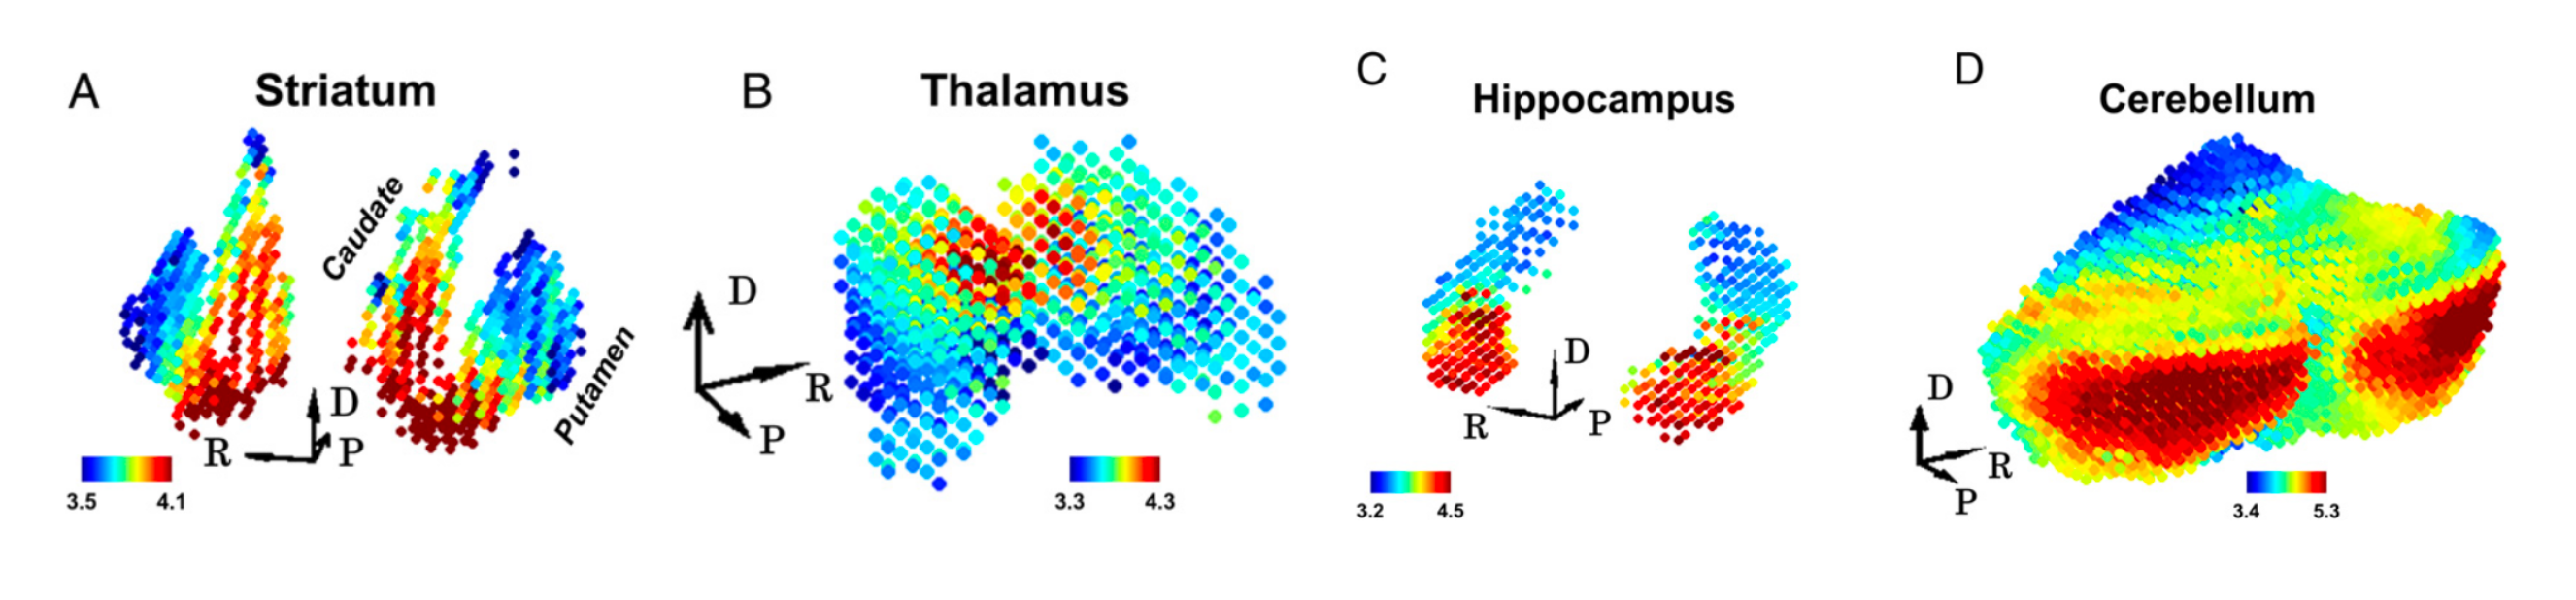
\includegraphics[width=0.95\textwidth]{latex/slides/raut-et-al.png}}
\end{frame}

% slide %
\begin{frame}{Timescale Functional Roles}
\footnotesize
\textbf{Experimental Conditions}
\begin{itemize}
    \item Pharmacological agents: Propofol (\cite{huang_timescales_2018}) and Serotonergic drugs (\cite{shinn_functional_2023}).
    \item Working memory tasks (\cite{gao_neuronal_2020}).
    \item Sleep deprivation (\cite{meisel_decline_2017}).
\end{itemize}
\vspace{0.25cm}
\textbf{Observational Studies}
\begin{itemize}
    \item Ageing (\cite{gao_neuronal_2020}).
    \item Psychiatric disorders: Autism (\cite{watanabe_atypical_2019}) and Schizophrenia (\cite{wengler_distinct_2020}).
\end{itemize}
\end{frame}

% slide % 
\begin{frame}{Recording Brain Activity}
\footnotesize
\vspace{0.25cm}
\textbf{Electrical Signals}: EEG, ECoG, iEEG
\begin{itemize}
    \item Dense sampling in time, sparse sampling in space.
\end{itemize}

\visible{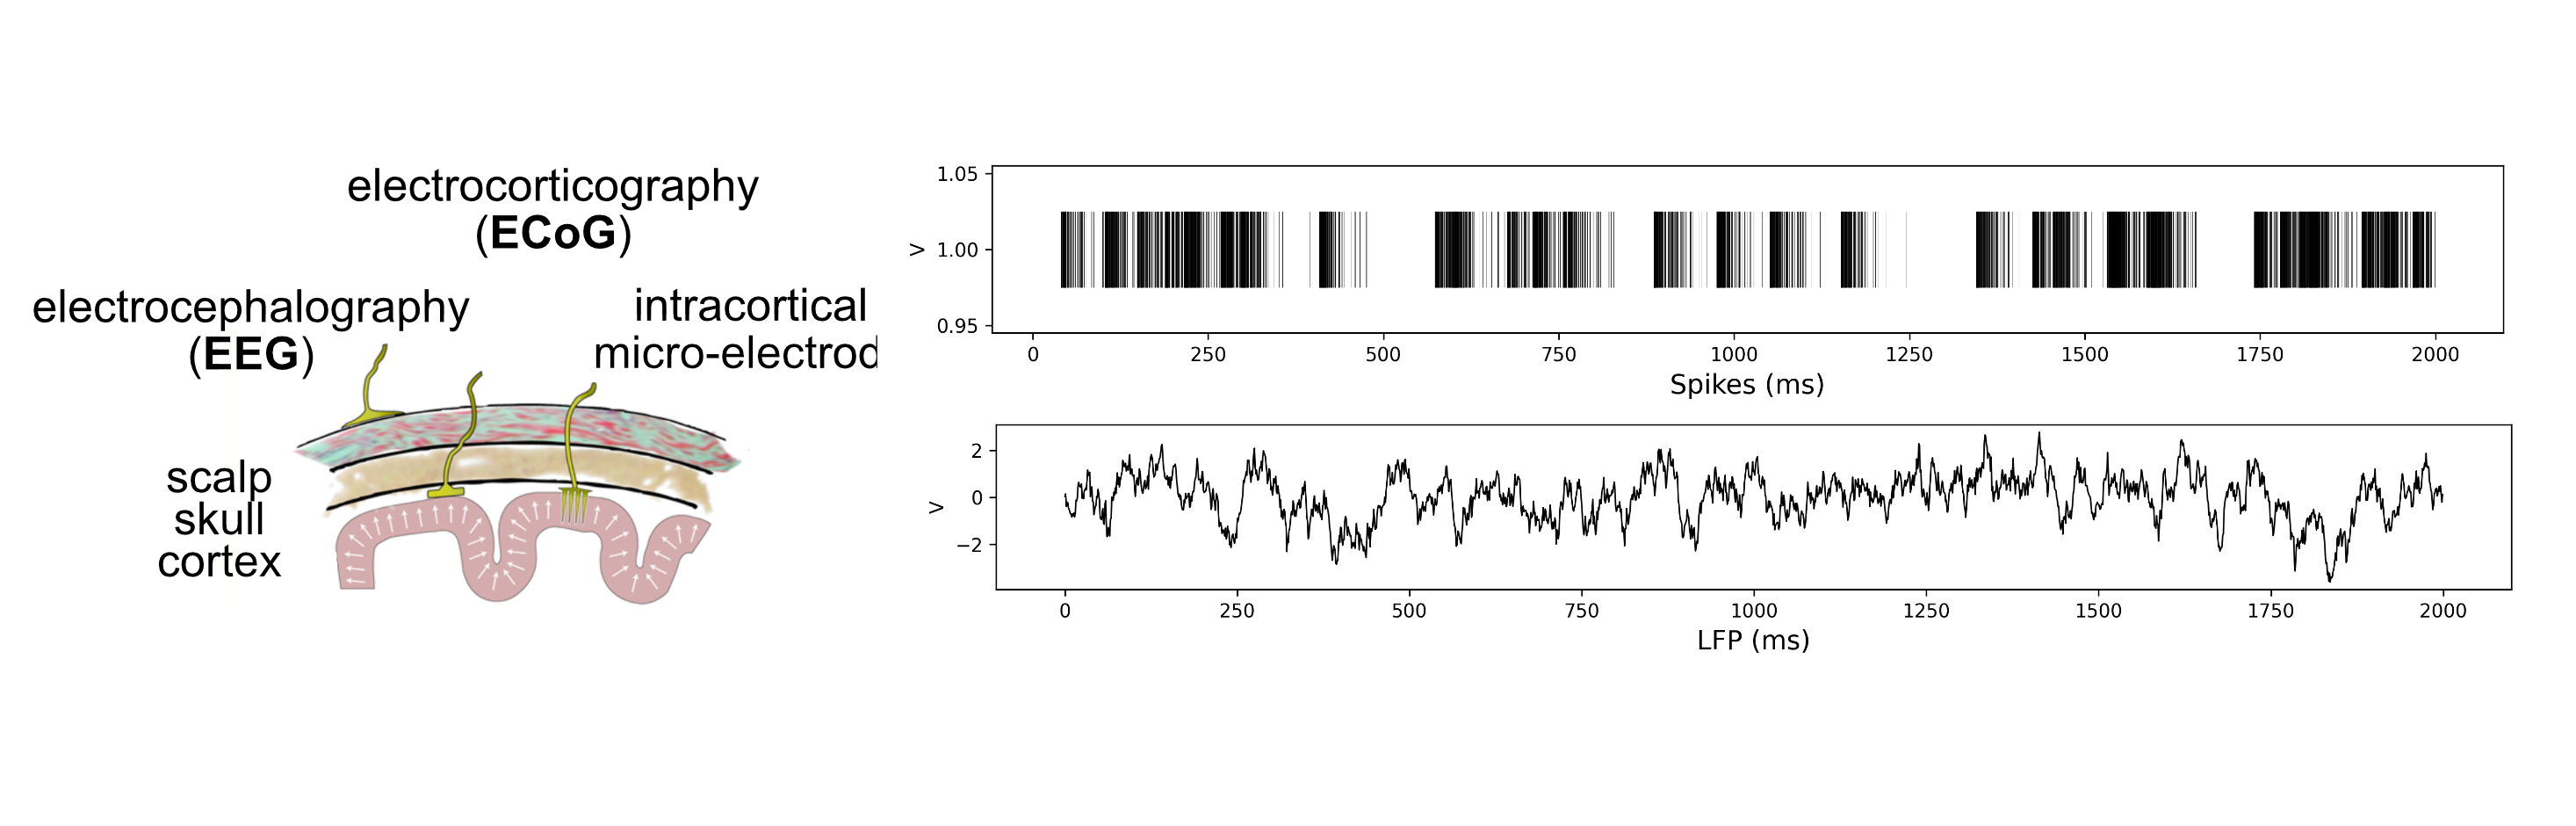
\includegraphics[width=1\textwidth]{latex/slides/eeg.png}}

\textbf{Hemodynamic Signals}: fMRI
\begin{itemize}
    \item Sparse sampling in time, dense sampling in space.
\end{itemize}
\visible{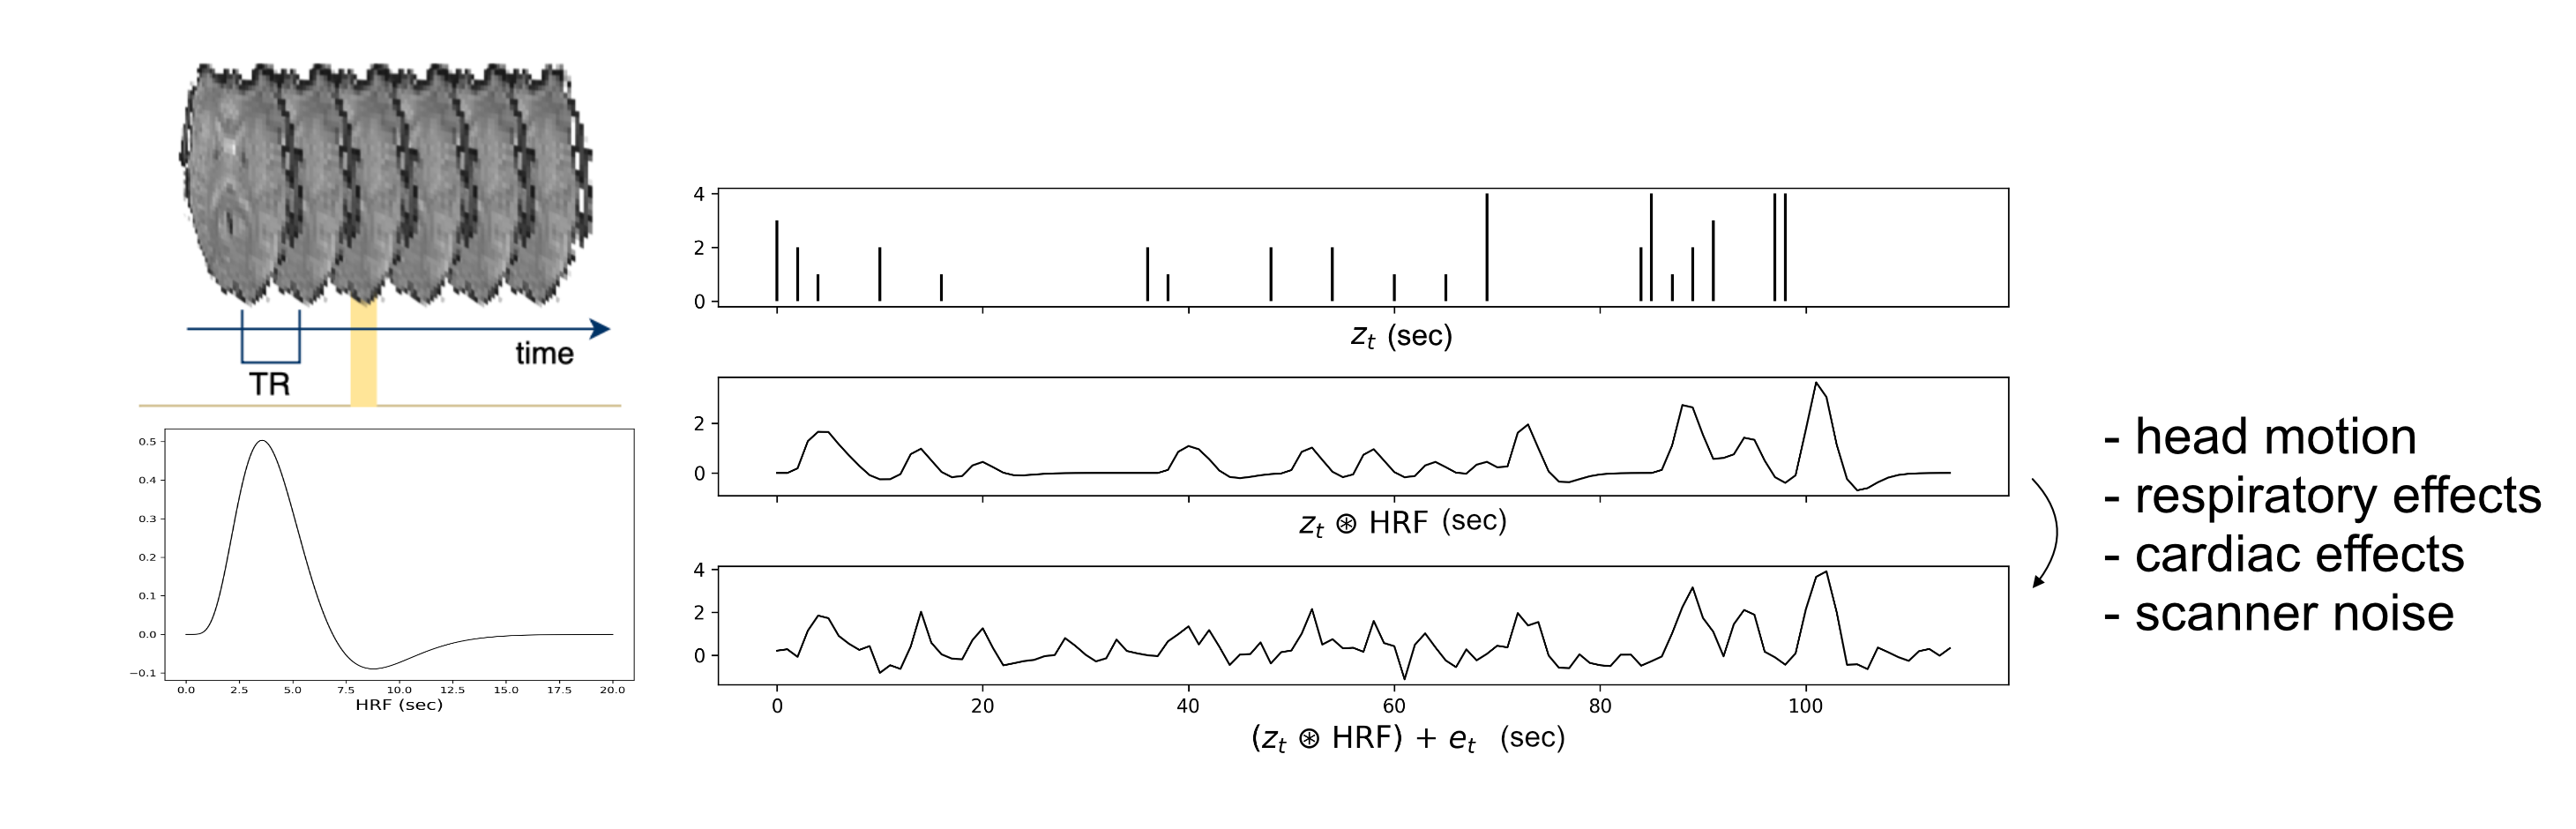
\includegraphics[width=1\textwidth]{latex/slides/hrf.png}}
\end{frame}

% slide % 
\begin{frame}{fMRI Timescale Maps}
\centering
\visible{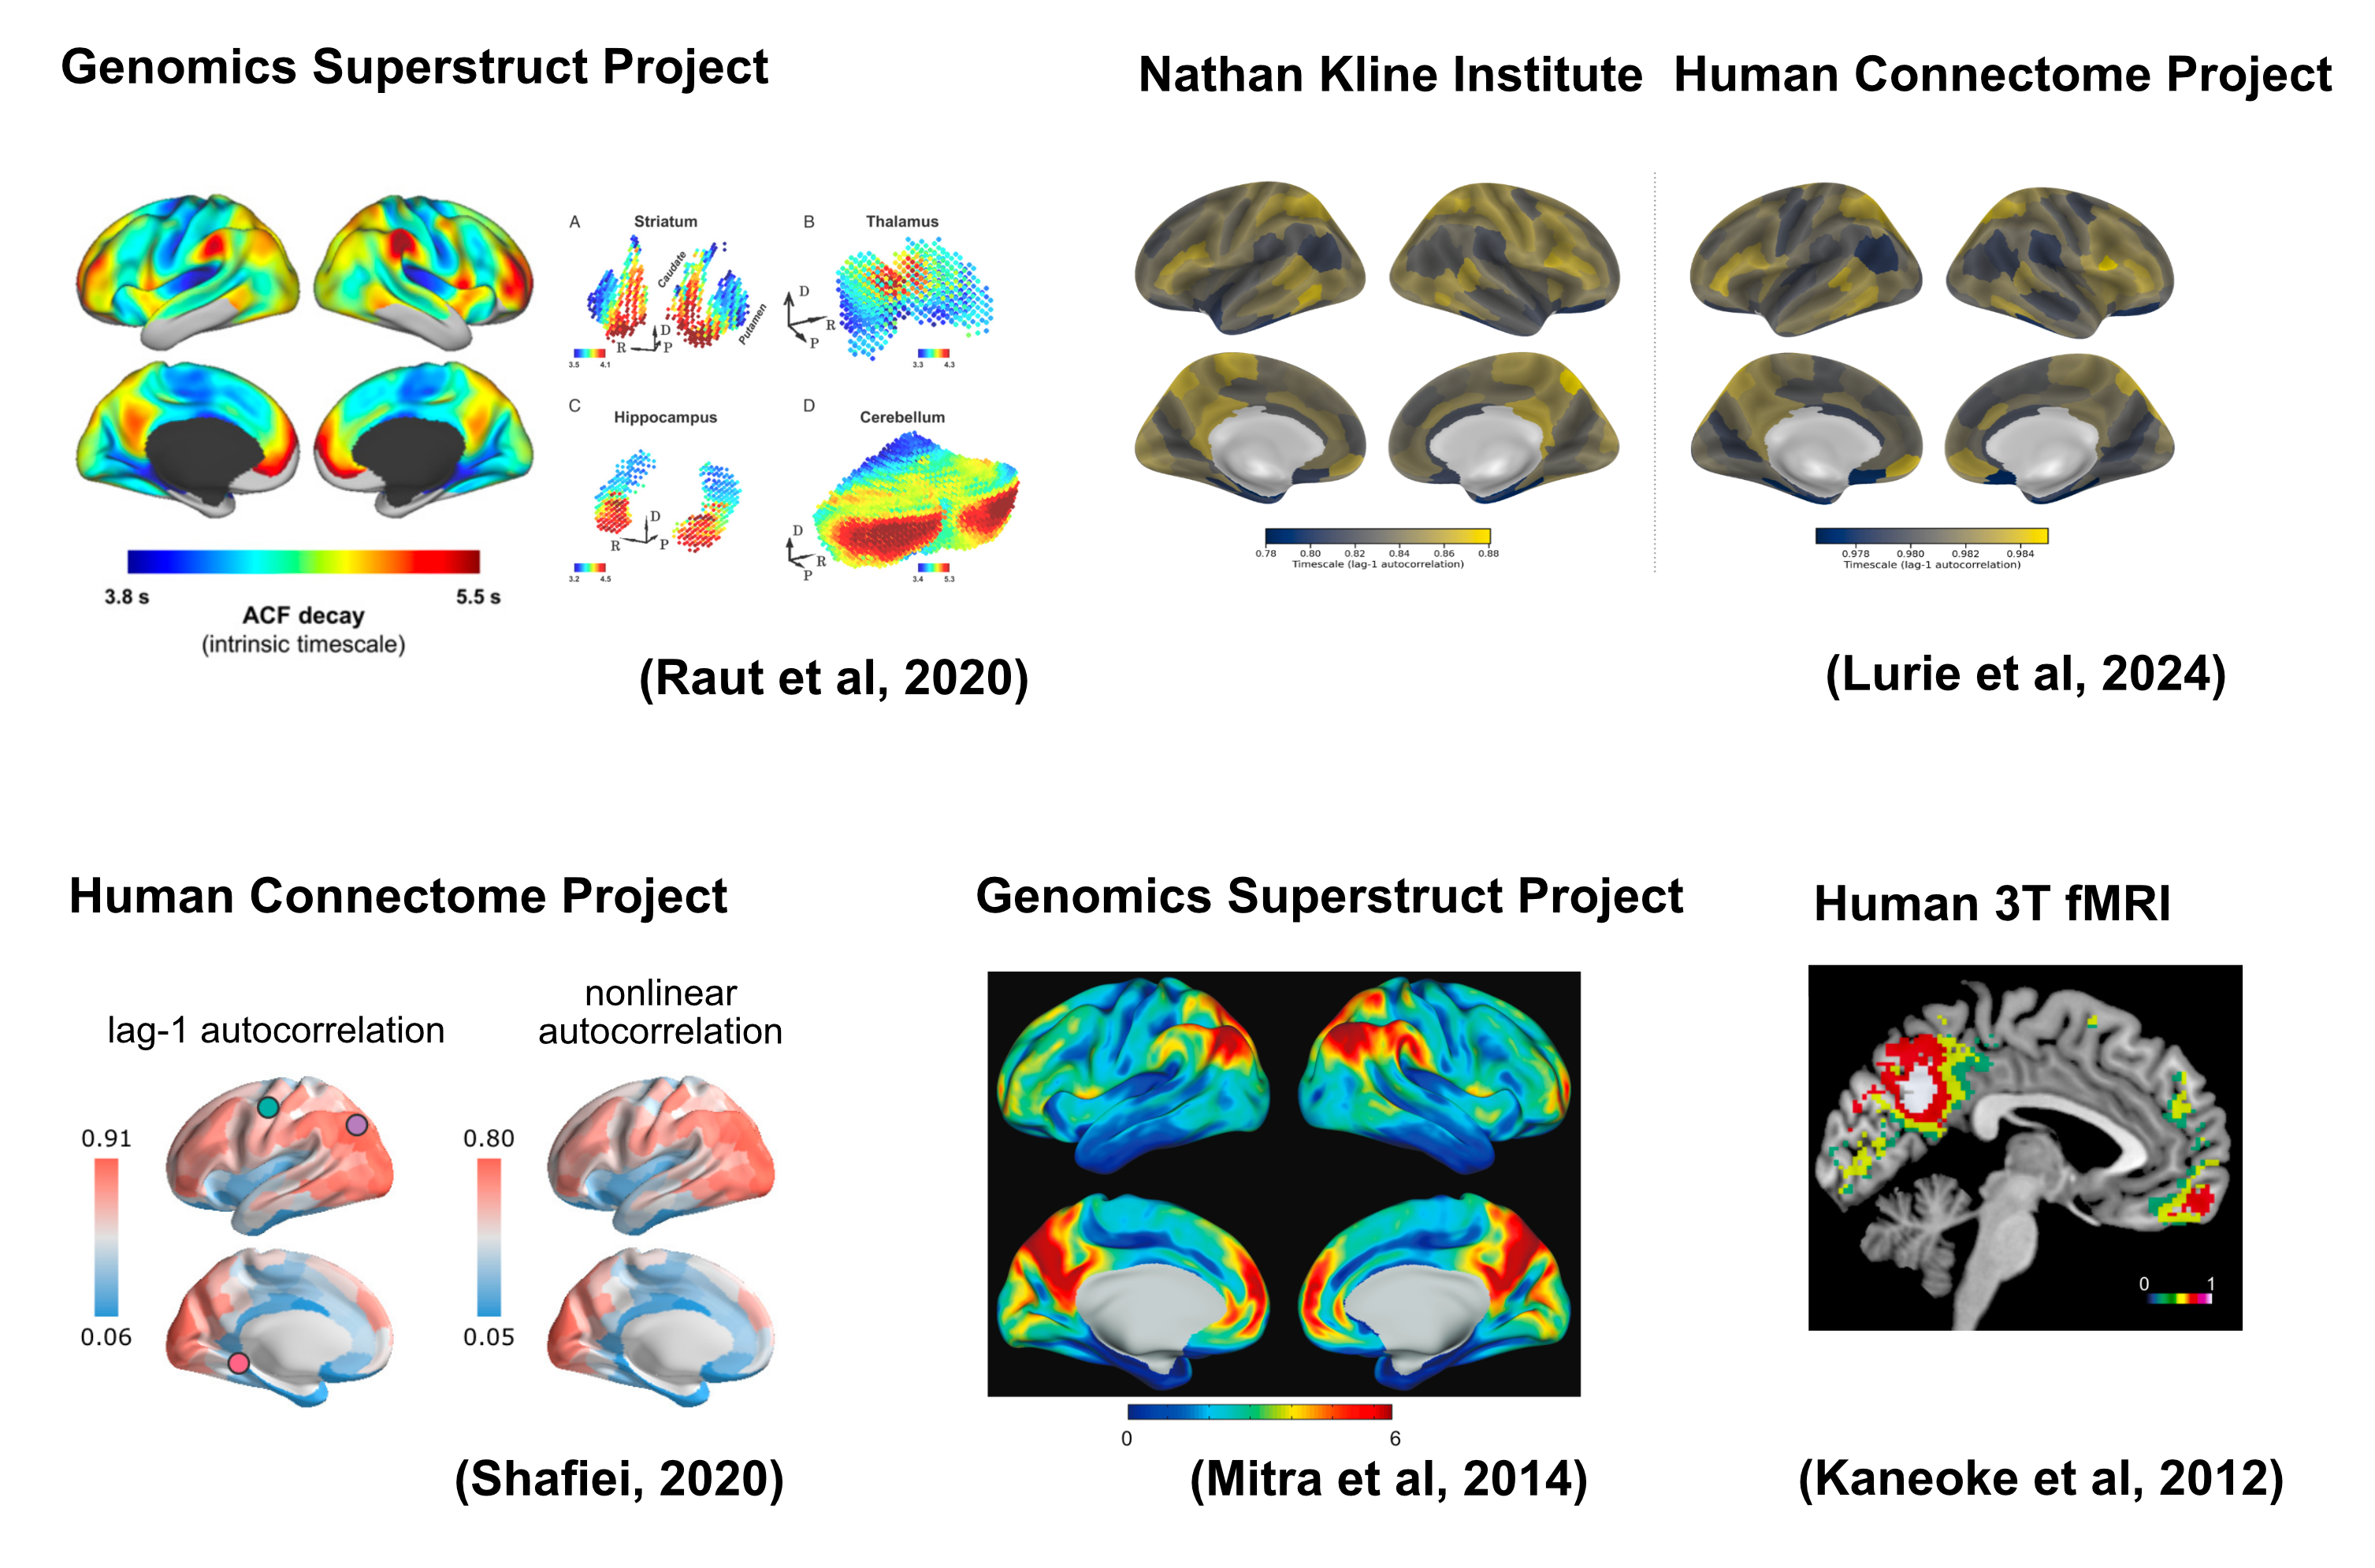
\includegraphics[width=1\textwidth]{latex/slides/fmri-maps01.png}}
\scriptsize
\cite{raut_hierarchical_2020, lurie_cortical_2024, shafiei_topographic_2020, mitra_lag_2014, kaneoke_variance_2012}
\end{frame}

% slide %
\begin{frame}{fMRI Timescale Maps}
\centering
\visible{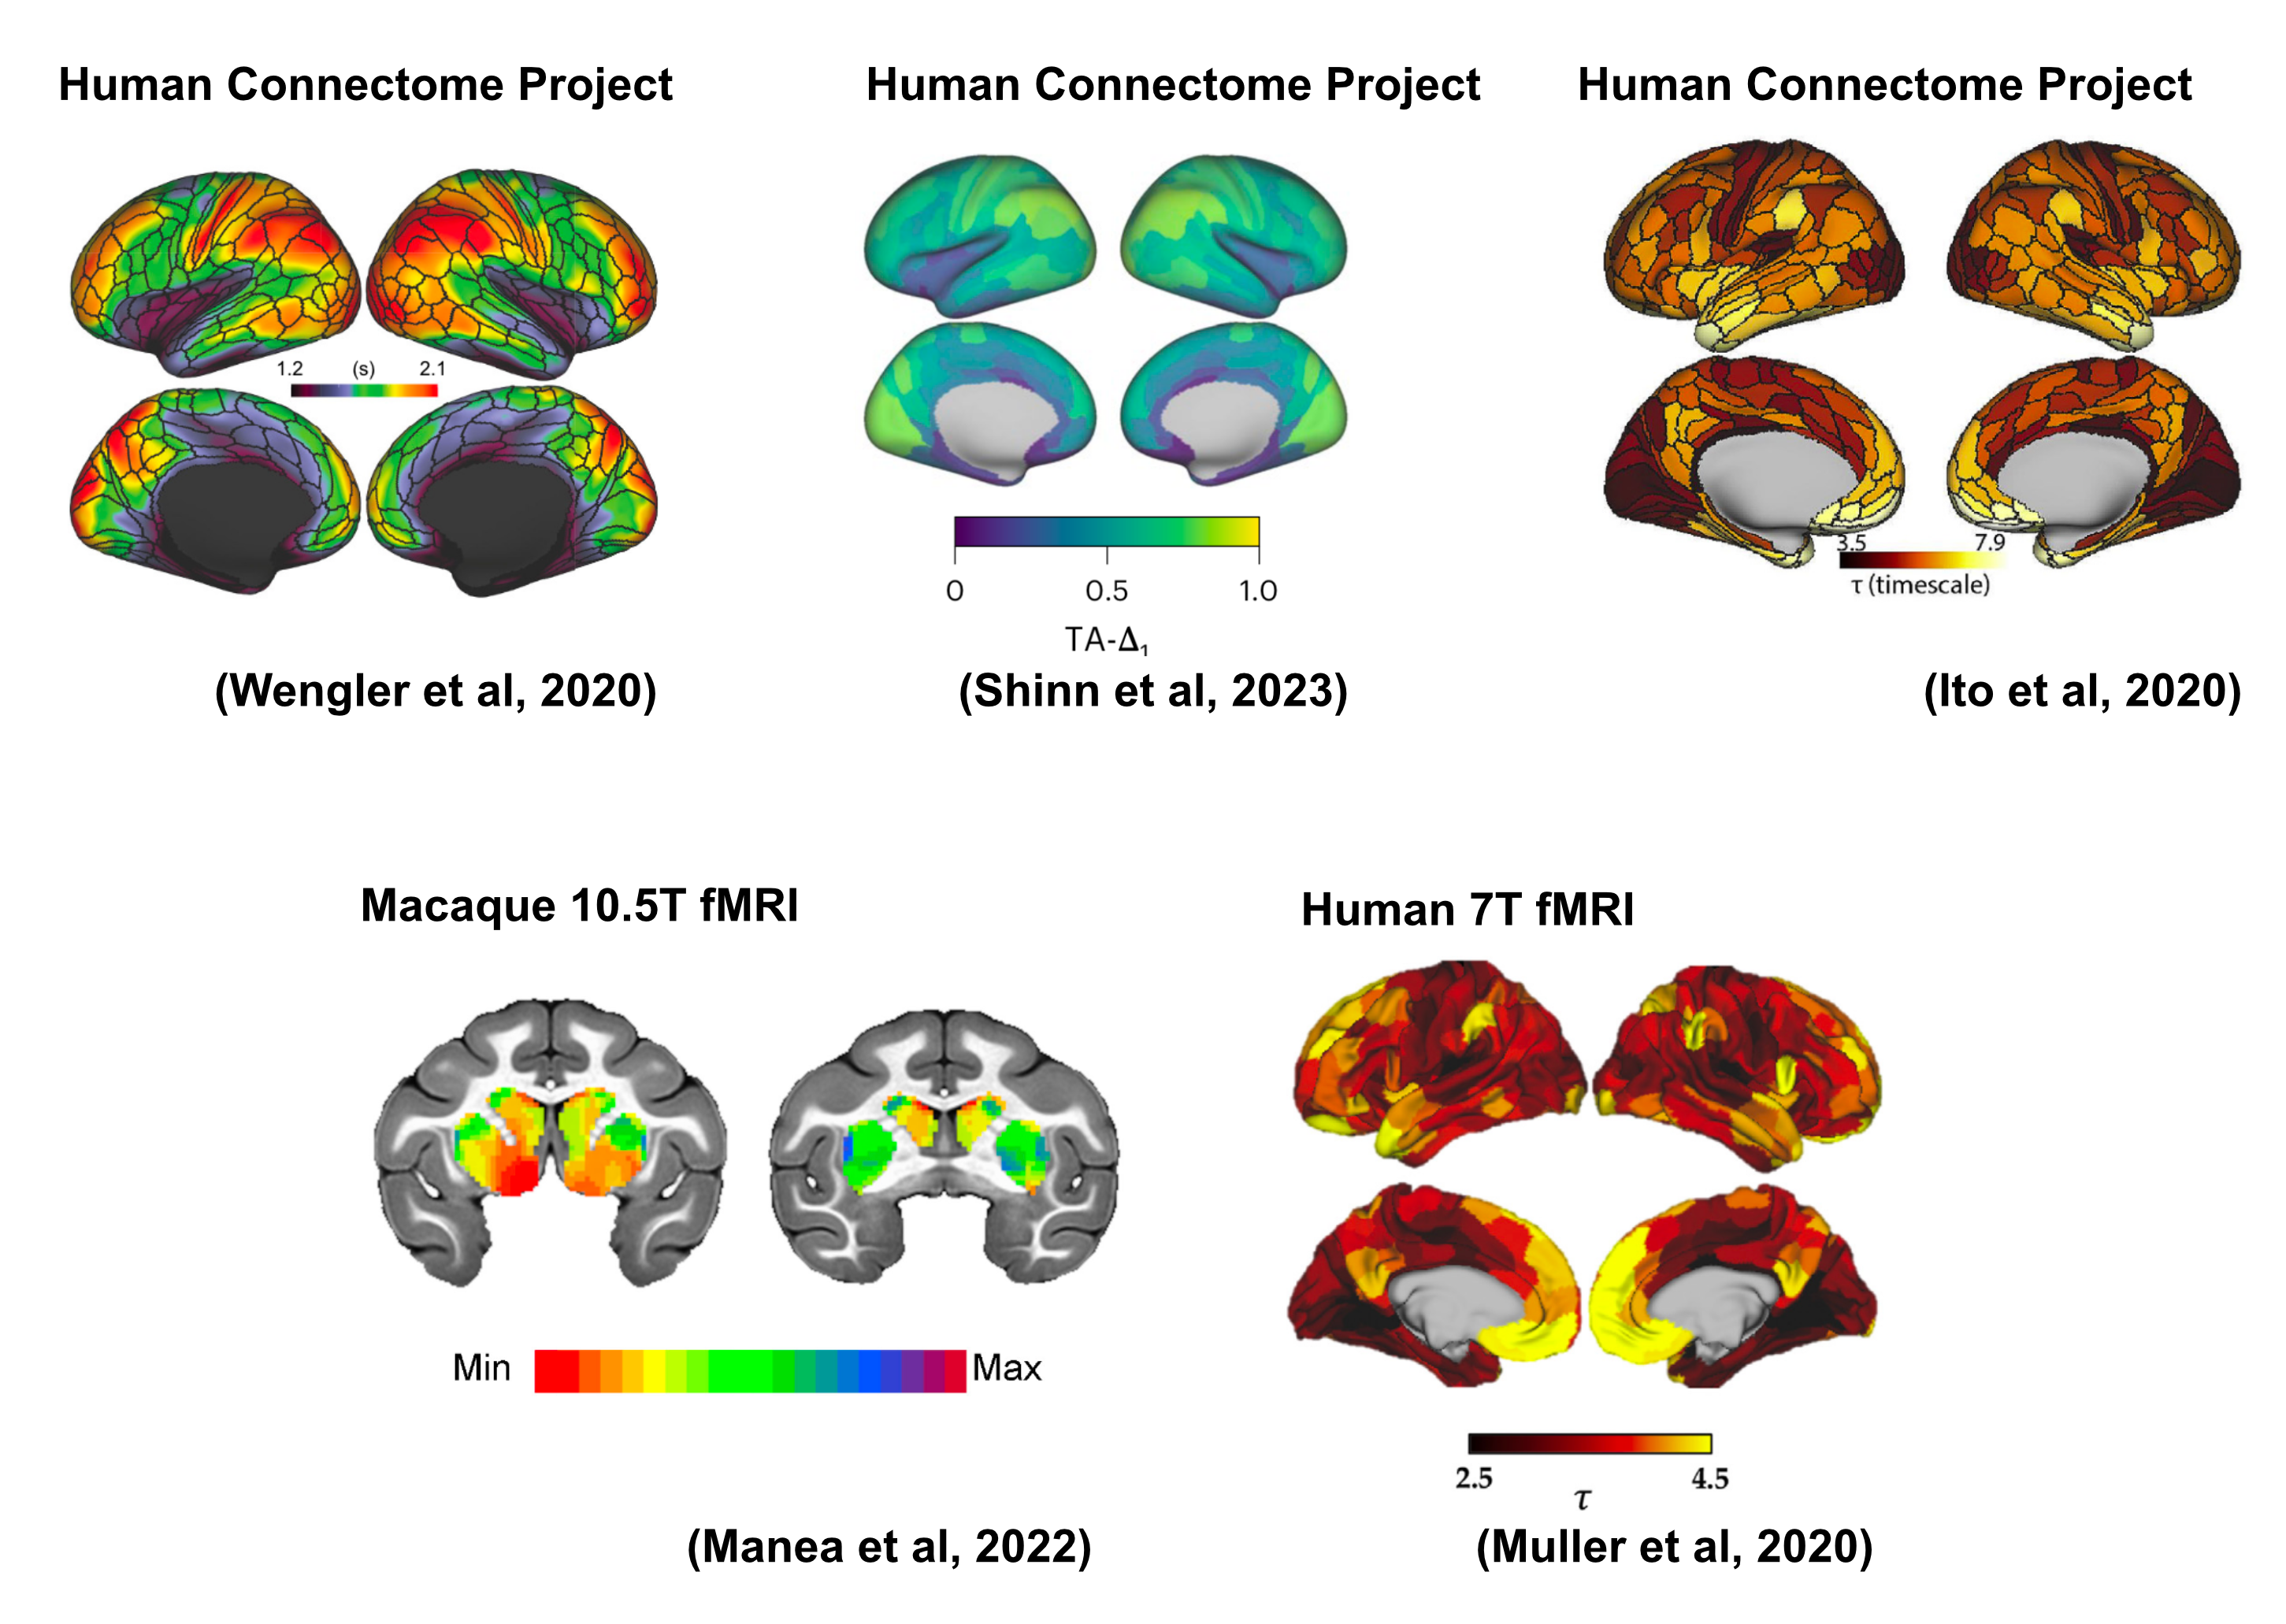
\includegraphics[width=1\textwidth]{latex/slides/fmri-maps02.png}}
\scriptsize
\cite{wengler_distinct_2020, shinn_functional_2023, ito_cortical_2020, manea_intrinsic_2022, muller_core_2020}
\end{frame}

% slide %
\subsection{Methodological}
\footnotesize
\begin{frame}{Timescale Methods}
\begin{enumerate}
    \item \textbf{Time Domain} (6/25 papers):\\
    \begin{scriptsize}
        \cite{kaneoke_variance_2012, meisel_decline_2017, huang_timescales_2018, lurie_cortical_2024, shinn_functional_2023, shafiei_topographic_2020}
    \end{scriptsize}
    \item \textbf{Autocorrelation Domain} (18/25 papers):\\
    \begin{scriptsize}
        \cite{murray_hierarchy_2014, rossi-pool_invariant_2021, cirillo_neural_2018, ito_cortical_2020, runyan_distinct_2017, zeraati_flexible_2022, nougaret_intrinsic_2021, wasmuht_intrinsic_2018, muller_core_2020, maisson_choice-relevant_2021, li_hierarchical_2022, shafiei_topographic_2020, wengler_distinct_2020, manea_intrinsic_2022, watanabe_atypical_2019, zilio_are_2021, raut_hierarchical_2020, golesorkhi_temporal_2021}
    \end{scriptsize}
    \item Frequency Domain (3/25 papers):\\
    \begin{scriptsize}
        \cite{gao_neuronal_2020, zeraati_flexible_2022, fallon_timescales_2020}
    \end{scriptsize}
\end{enumerate}
\end{frame}

% slide %
\begin{frame}{Project Objective}
\footnotesize
\textbf{Problem Statement}:
\begin{itemize}
    \item Current timescale methods rely on restrictive assumptions about the underlying stochastic process
    \item Existing research reports point estimates without standard errors, hindering accurate inference and comparisons across brain regions
\end{itemize}
\textbf{Proposed Solution}:
\begin{itemize}
    \item Build on existing methods, designed to be robust under general assumptions
    \item Analyze the statistical properties (bias, consistency, limiting variance) of these estimators
\end{itemize}
\end{frame}

\section{Definitions}

% slide %
\subsection{Assumptions}
\begin{frame}{Assumptions}
\footnotesize
Let $\{X_t, t\in \mathbb{Z}\}$ be a discrete stochastic process that is \textbf{weakly stationary} and \textbf{ergodic}, and $x_t = \{x_1, x_2, ..., x_T\}$ be a finite sample. Assume $X_t$ and $x_t$ are mean zero.\\
\vspace{0.25cm}
\textbf{Stationarity implies}:
\begin{align}
    \gamma_k &= \text{cov}[X_t, X_{t-k}] = \mathbb{E}[X_t X_{t-k}]
\end{align}

\textbf{Ergodicity implies}:
\begin{align}
    \underset{T\to\infty}{\text{lim}} \frac{1}{T} \sum_{k=1}^T |\gamma_k| &= 0
\end{align}
(\cite{hansen_econometrics_2022})\\
\end{frame}

% slide %
\subsection{Models}
\begin{frame}{Autoregressive Model}
\footnotesize
Example of time domain method.
\vspace{0.25cm}

\textbf{Def. Autoregressive Model}
\begin{align}
    X_t = \phi X_{t-1} + e_t
\end{align}

\onslide<2->
\textbf{Def. Timescale}
\begin{align}
    \phi &= (\mathbb{E}[X_{t-1}^2])^{-1}(\mathbb{E}[X_t X_{t-1}])\\
    \tau &= g(\phi) = -\frac{1}{\text{log}(|\phi|)}. \label{eq:ar1-tau}
\end{align}
\vspace{0.25cm}

Implies a theoretical ACF that decays exponentially with a rate determined by $\phi$: $\rho_k = \phi^k$.\\
\vspace{0.25cm}
$\tau$ determines where the autocorrelations reach $1/{\textit{e}} \approx 0.37$.
\end{frame}

% slide %
\begin{frame}{Autoregressive Model}
\footnotesize
\textbf{Def. Standard Error of Timescale}:
\begin{align}
    \text{se}_\text{NW}(\phi) &= \sqrt{q^{-1} \omega q{-1}}\\
    \text{se}_\text{NW}(\tau) &\approx \text{se}_\text{NW}(\phi) \frac{d}{d\phi}g(\phi)
\end{align}

where:

\begin{align*}
    q &= \mathbb{E}[X_{t-1}^2]\\
    \omega &= \sum_{\ell=-\infty}^{\infty} \mathbb{E}[(X_{t-1}e_t)(X_{t-1-\ell}e_{t-\ell})]
\end{align*}
\cite{newey_simple_1987}
\end{frame}

\begin{frame}{Exponential Decay Model}
\footnotesize
Example of autocorrelation domain method.
\vspace{0.25cm}

\textbf{Def. Autocorrelation Function}:
\begin{align}
    \rho_k = \text{corr}(X_t, X_{t-k}) = \frac{\gamma_k}{\gamma_0}
\end{align}

\onslide<2->
\textbf{Def. Exponential Decay Model}:
\begin{align} \label{eq:acf}
\rho_k &= \phi^k + e_k
\end{align}

\onslide<3->
\textbf{Def. Timescale}: 
\begin{align}
    S(\phi) &= \mathbb{E}[(\rho_k - \phi^k)^2]\\
    \phi^* &= \underset{\phi}{\text{argmin }} S(\phi)\\
    \tau^* &= g(\phi^*) = -\frac{1}{\text{log}(|\phi^*|)}
\end{align}

$\tau^*$ determines where the autocorrelations reach $1/\textit{e} \approx 0.37$\\
(\cite{murray_hierarchy_2014})

\end{frame}

% slide %
\begin{frame}{Exponential Decay Model}
\footnotesize
\textbf{Def. Standard Error of Timescale}:
\begin{align}
    \text{se}_\text{NW}(\phi^*) &= \sqrt{q^{-1} \omega q^{-1}}\\
    \text{se}_\text{NW}(\tau^*) &\approx \text{se}_\text{NW}(\phi^*) \frac{d}{d\phi}g(\phi^*)
\end{align}

where:
\begin{align*}
    m(k, \phi) &= \phi^k\\
    m_{\phi, k} &= \frac{d}{d\phi} m(k, \phi) = k \phi ^{k-1}\\
    q &= \mathbb{E}[m_{\phi^*, k}^2] = \mathbb{E}[(k \phi^{*k-1})^2]\\
    \omega &= \sum_{\ell=-\infty}^{\infty} \mathbb{E}[(m_{\phi^*, k} e_{k})(m_{\phi^*, k-\ell} e_{k-\ell})]
\end{align*}
(\cite{newey_simple_1987})
\end{frame}

% slide %
\subsection{Estimators}
\begin{frame}{Least Squares Methods}
Autoregressive Model \textbf{Linear/Ordinary Least Squares}:\\
\begin{center}
    \visible{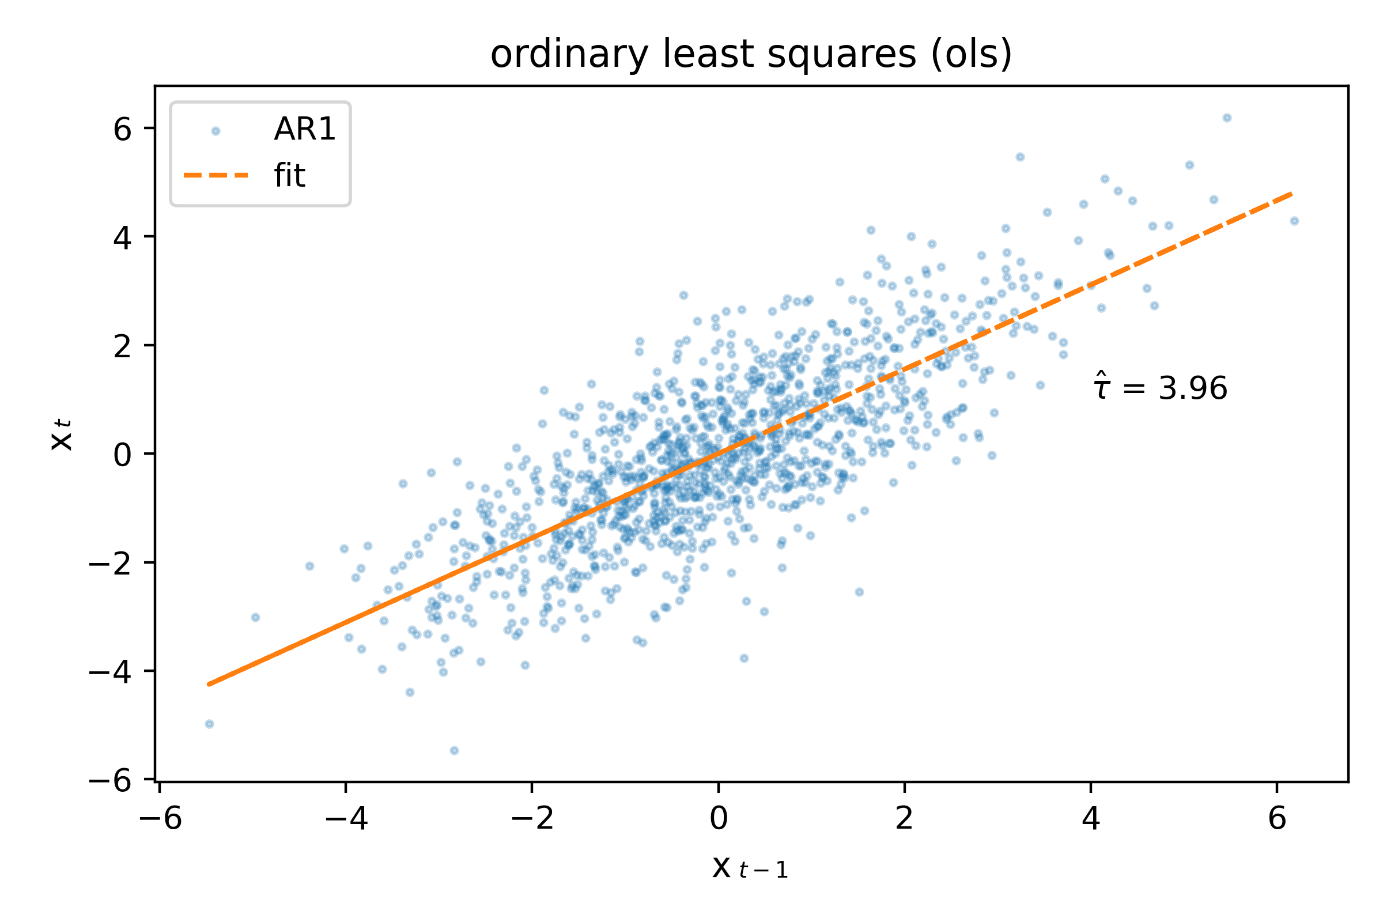
\includegraphics[width=0.6\textwidth]{latex/slides/ols.png}}
\end{center}

Exponential Decay Model \textbf{Nonlinear Least Squares}:\\
\vspace{0.25cm}
\begin{center}
    \visible{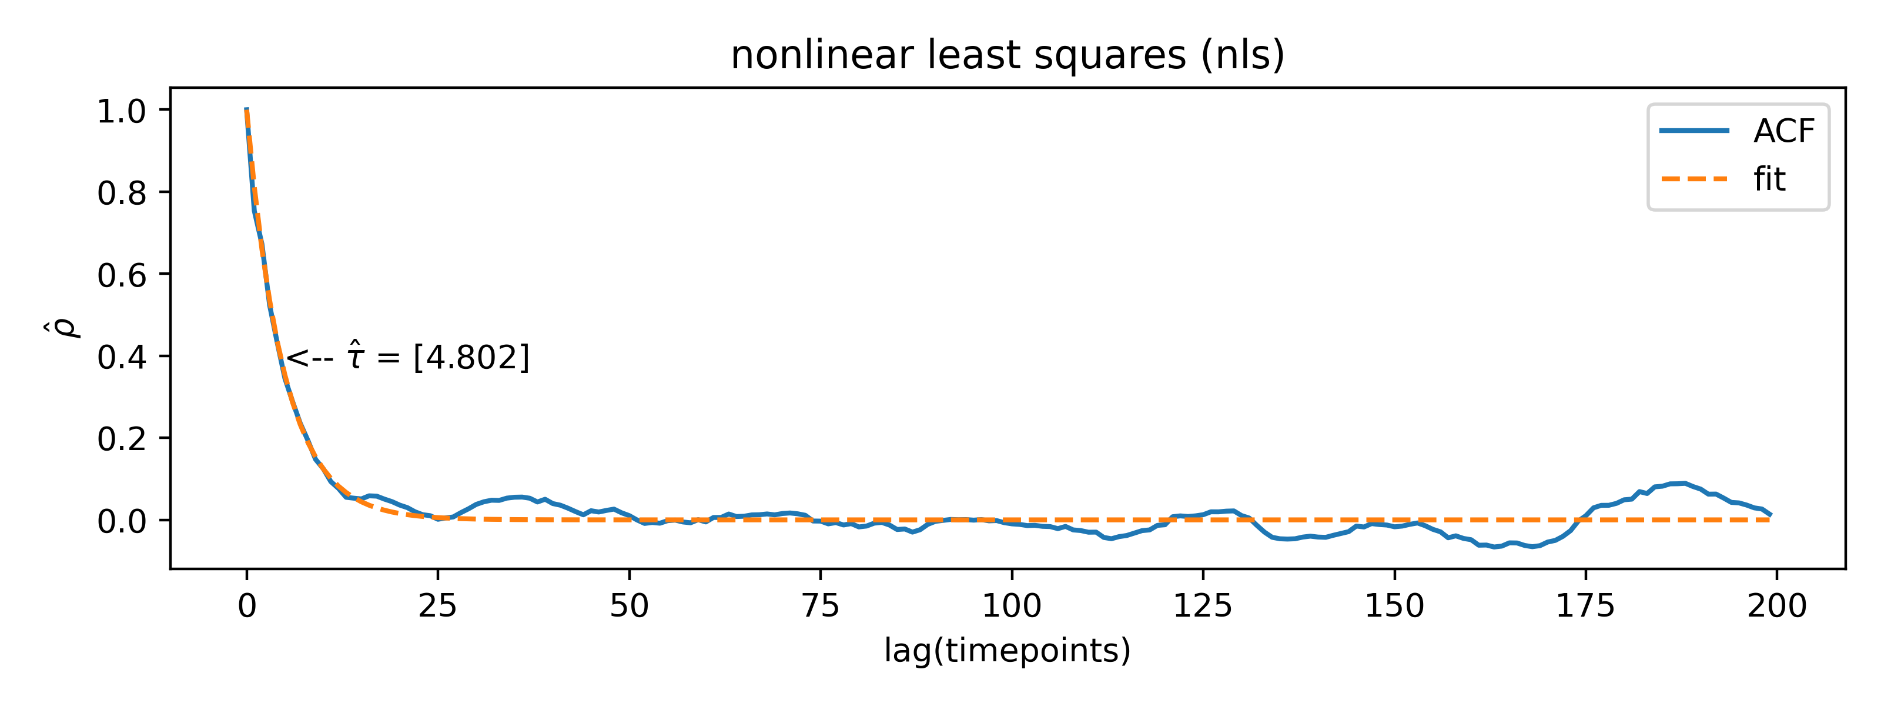
\includegraphics[width=0.9\textwidth]{latex/slides/nls.png}}
\end{center}
\end{frame}


% slide %
\begin{frame}{Estimation of Autoregressive Model}
\footnotesize

\textbf{Est: Linear Least Squares}
\begin{align}
    \hat\phi &= (\sum_{t=2}^T x_{t-1}^2)^{-1} (\sum_{t=2}^T x_t x_{t-1})\\
    \hat\tau &= g(\hat\phi) = -\frac{1}{\text{log}(|\hat\phi|)}
\end{align}

\onslide<2->
\textbf{Est: Standard Error}
\begin{align}
    \text{se}_\text{NW}(\hat\phi) &= \sqrt{\hat q^{-1}\hat\omega\hat q^{-1}}\\
    \text{se}_\text{NW}(\hat\tau) &= \text{se}_\text{NW}(\hat\phi) \frac{d}{d\phi} g(\hat\phi)
\end{align}

\end{frame}


% slide %
\begin{frame}{Estimation of Exponential Decay Model}
\footnotesize

\textbf{Est: Autocorrelation Function}
\begin{align}
    \hat\rho_k &= (\hat\gamma_0)^{-1}(\hat\gamma_k) = (\sum_{t=1}^T x_t^2)^{-1} (\sum_{t=k+1}^{T}x_t x_{t-k})
\end{align}

\onslide<2->
\textbf{Est: Nonlinear Least Squares}
\begin{align}
    \hat S(\phi) &= \frac{1}{K} \sum_{k=1}^K (\hat\rho_k - \phi^k)^2\\
    \hat\phi^* &= \underset{\phi}{\text{argmin }} \hat S(\phi)\\
    \hat\tau^* &= g(\hat\phi^*) = -\frac{1}{\text{log}(|\hat\phi^*|)}
\end{align}

\onslide<3->
\textbf{Est: Standard Error}
\begin{align}
    \text{se}_\text{NW}(\hat\phi) &= \sqrt{\hat q^{-1}\hat\omega\hat q^{-1}}\\
    \text{se}_\text{NW}(\hat\tau) &= \text{se}_\text{NW}(\hat\phi) \frac{d}{d\phi} g(\hat\phi)
\end{align}
\end{frame}


\section{Simulations}

% slide %
\subsection{AR-1}
\begin{frame}{AR-1 Simulation}
\footnotesize
\begin{itemize}
    \item \textbf{Setting}: $T = 4800$ timepoints, $N = 1000$ repeats.
    \item \textbf{AR process}: $x_t = {\phi} x_{t-1} + e_t, \quad e_t \overset{iid}{\sim} \mathcal{N}(0, 1)$
    \item \textbf{Parameters}:\\
    $\phi \in \{\textcolor[HTML]{000000}{0.1}, \textcolor[HTML]{B66B7C}{0.28}, \textcolor[HTML]{8D9FCB}{0.45}, \textcolor[HTML]{66C2A6}{0.62}, \textcolor[HTML]{7D7D7D}{0.8}\}$\\
\end{itemize}

\centering
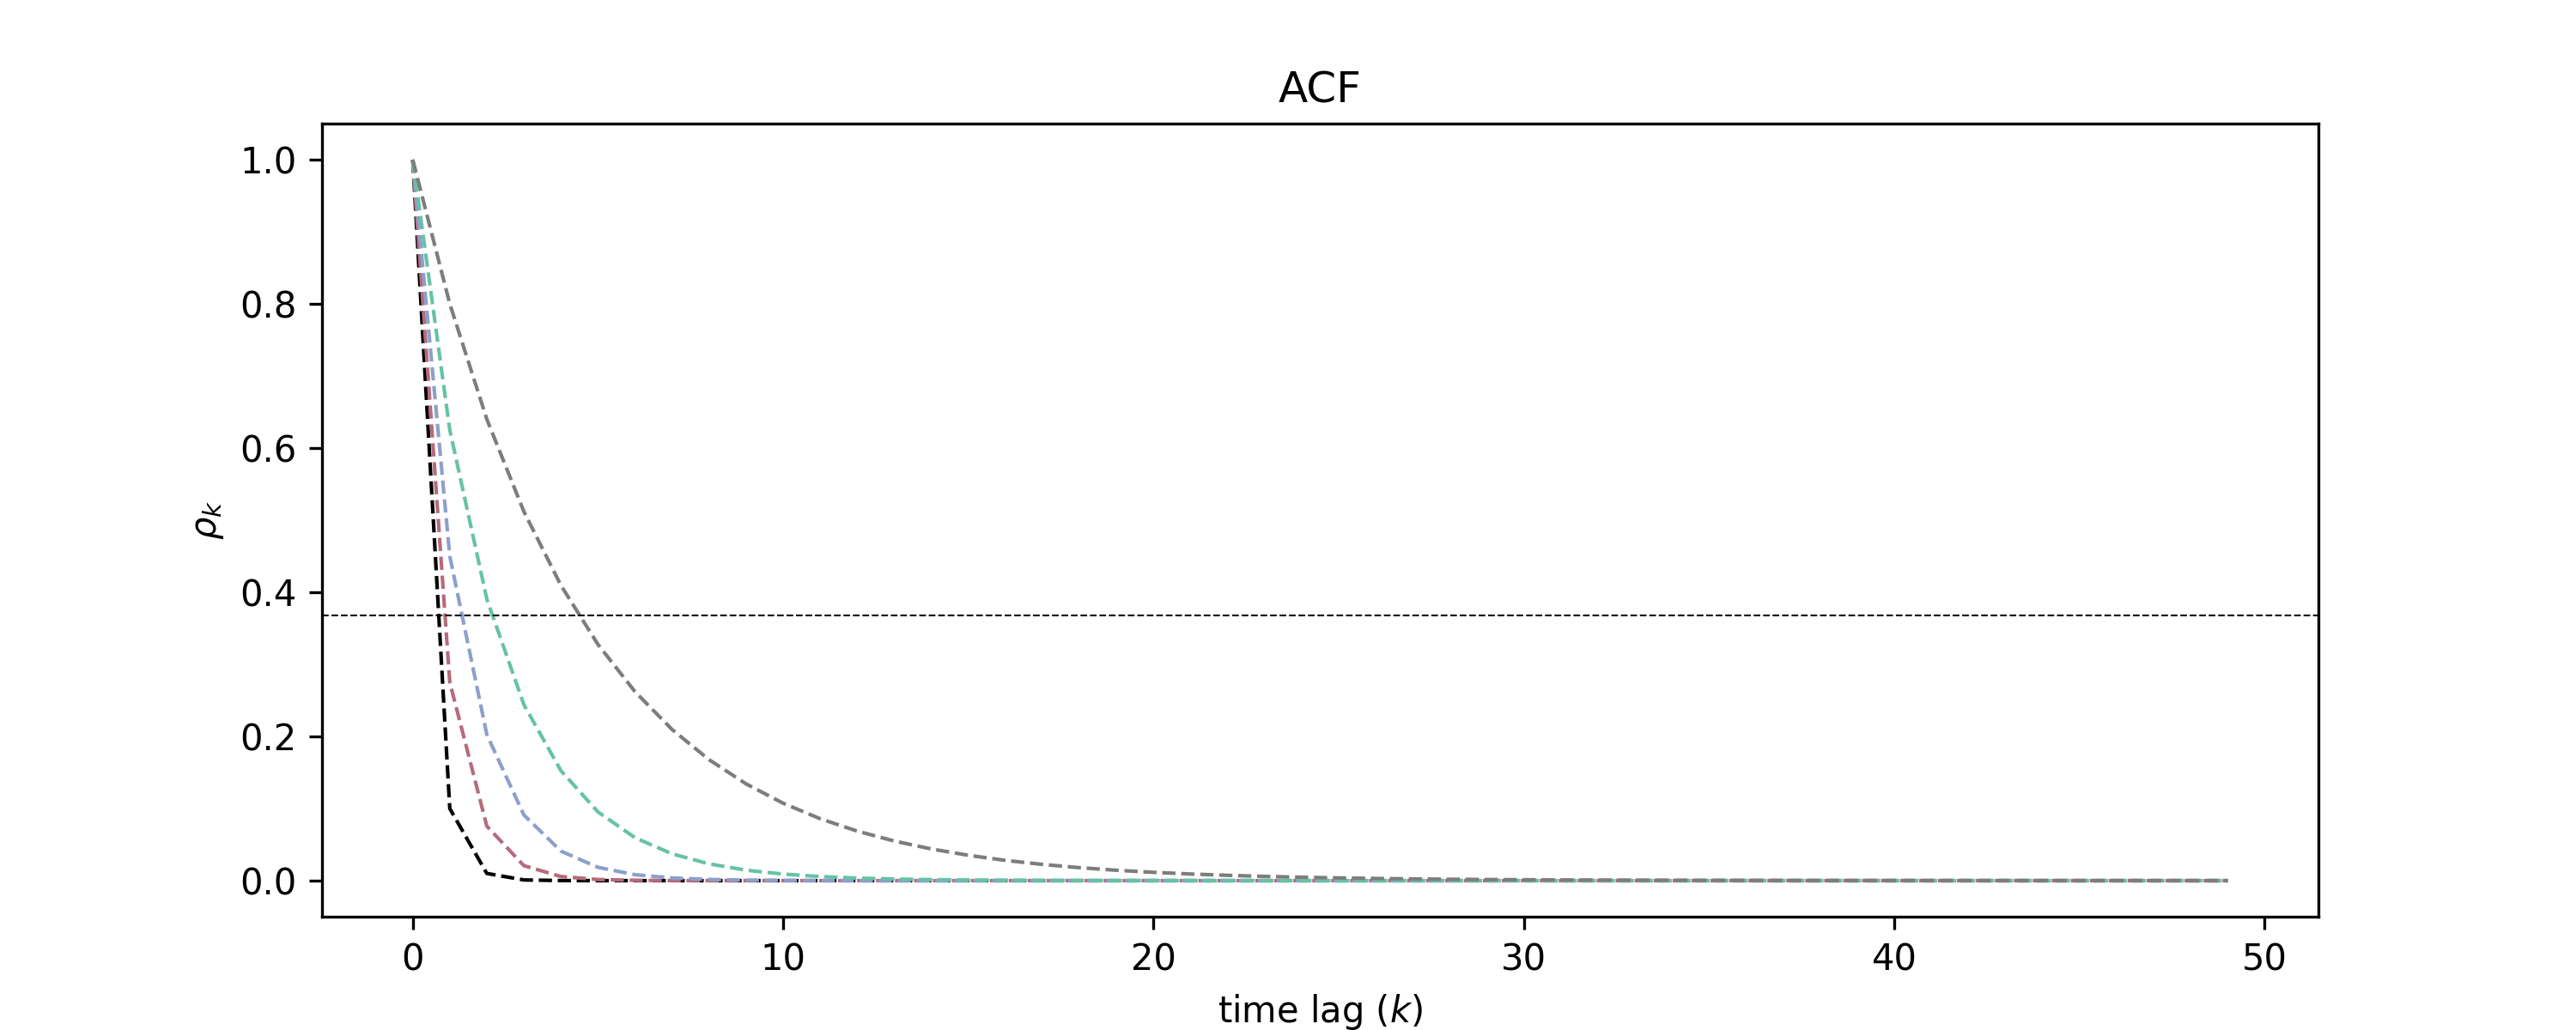
\includegraphics[width=0.9\textwidth]{latex/slides/simulations-ar1.png}
\end{frame}

% slide % 
\begin{frame}{AR-1 Results}
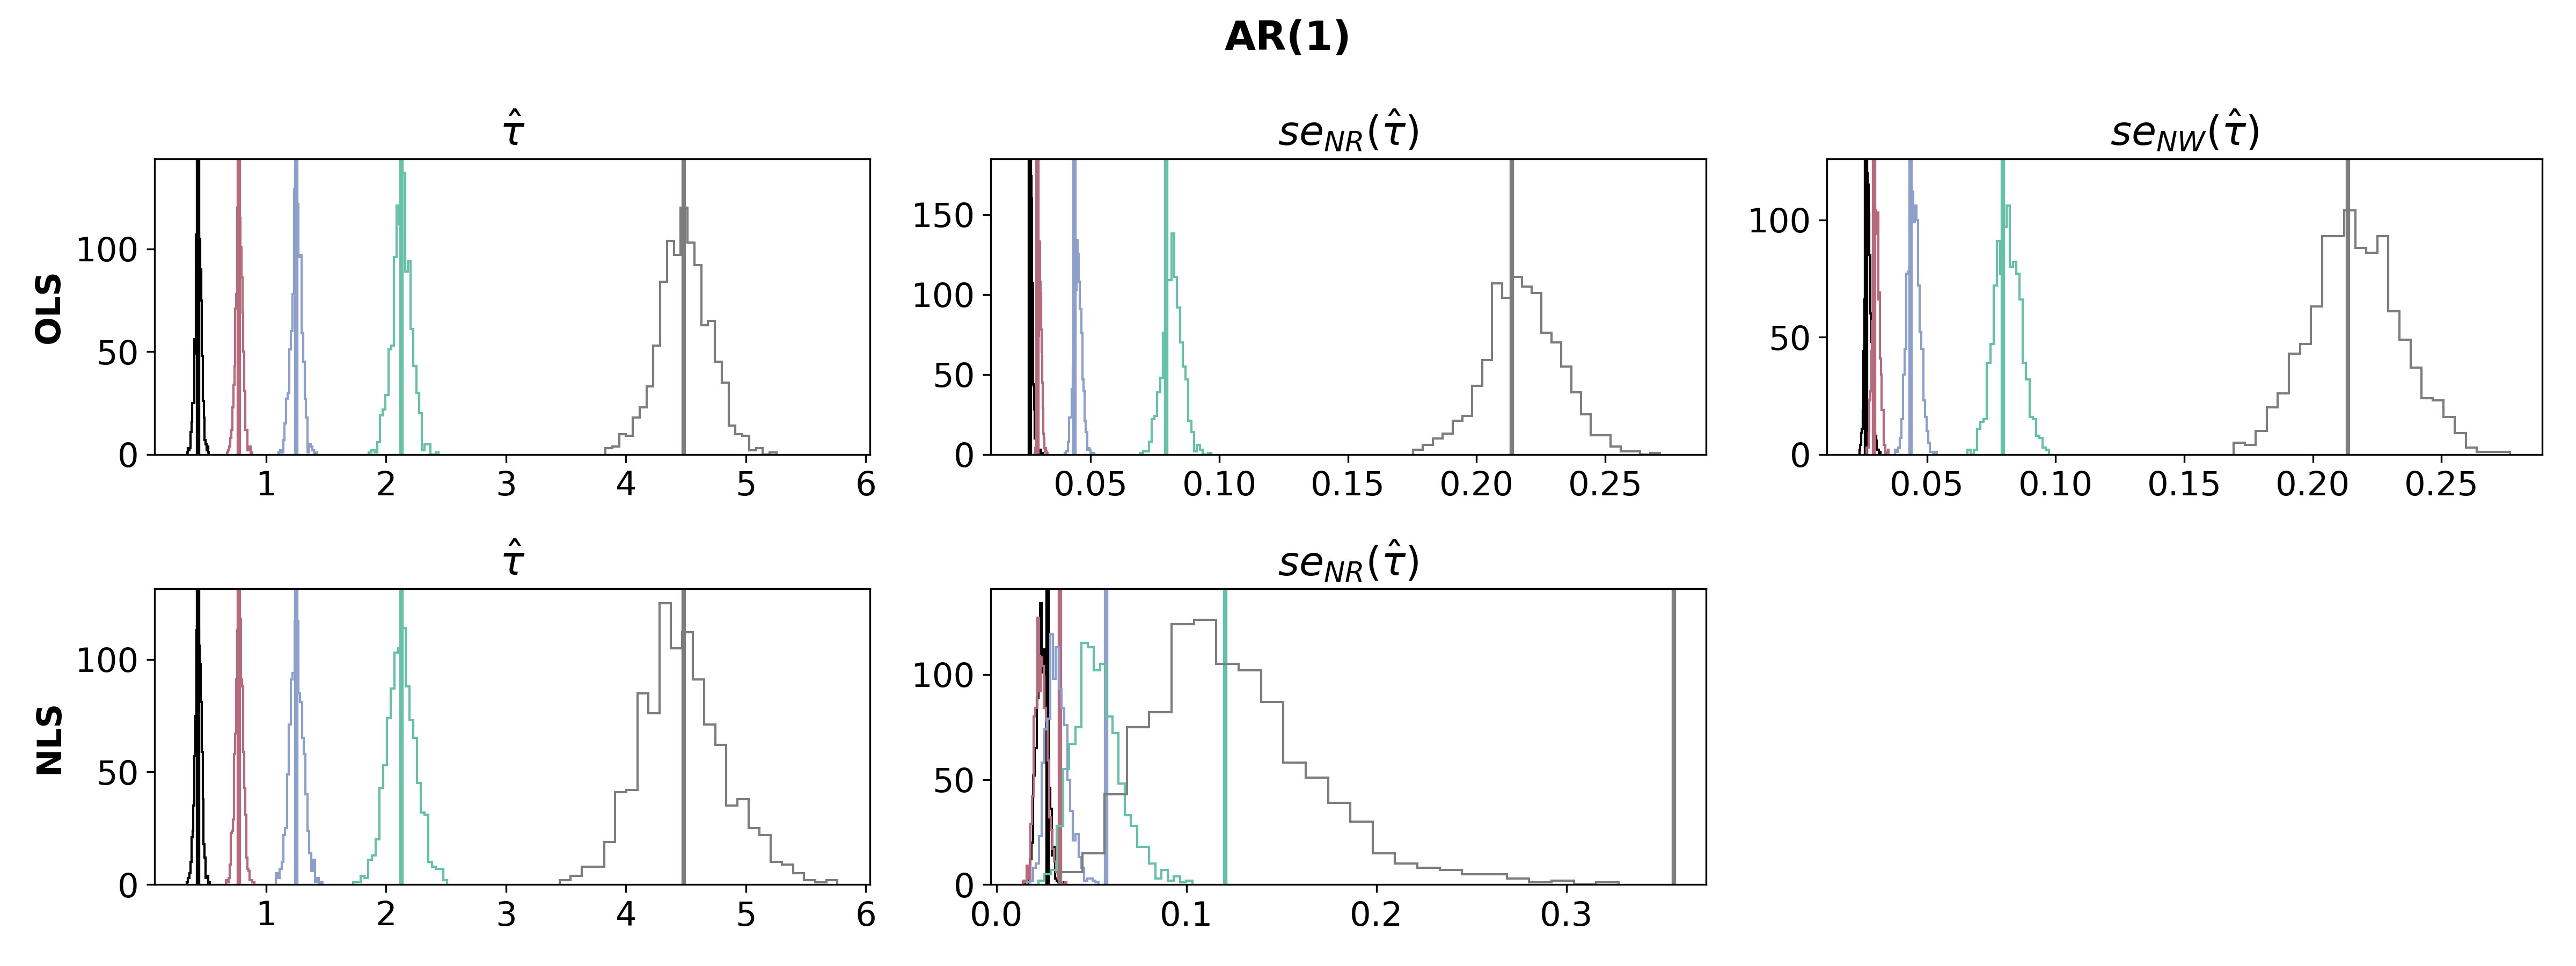
\includegraphics[width=1\textwidth]{latex/slides/sim-ar1.png}
\end{frame}

% slide %
\subsection{AR-2}
\begin{frame}{AR-2 Stationarity Conditions}
\centering
\visible{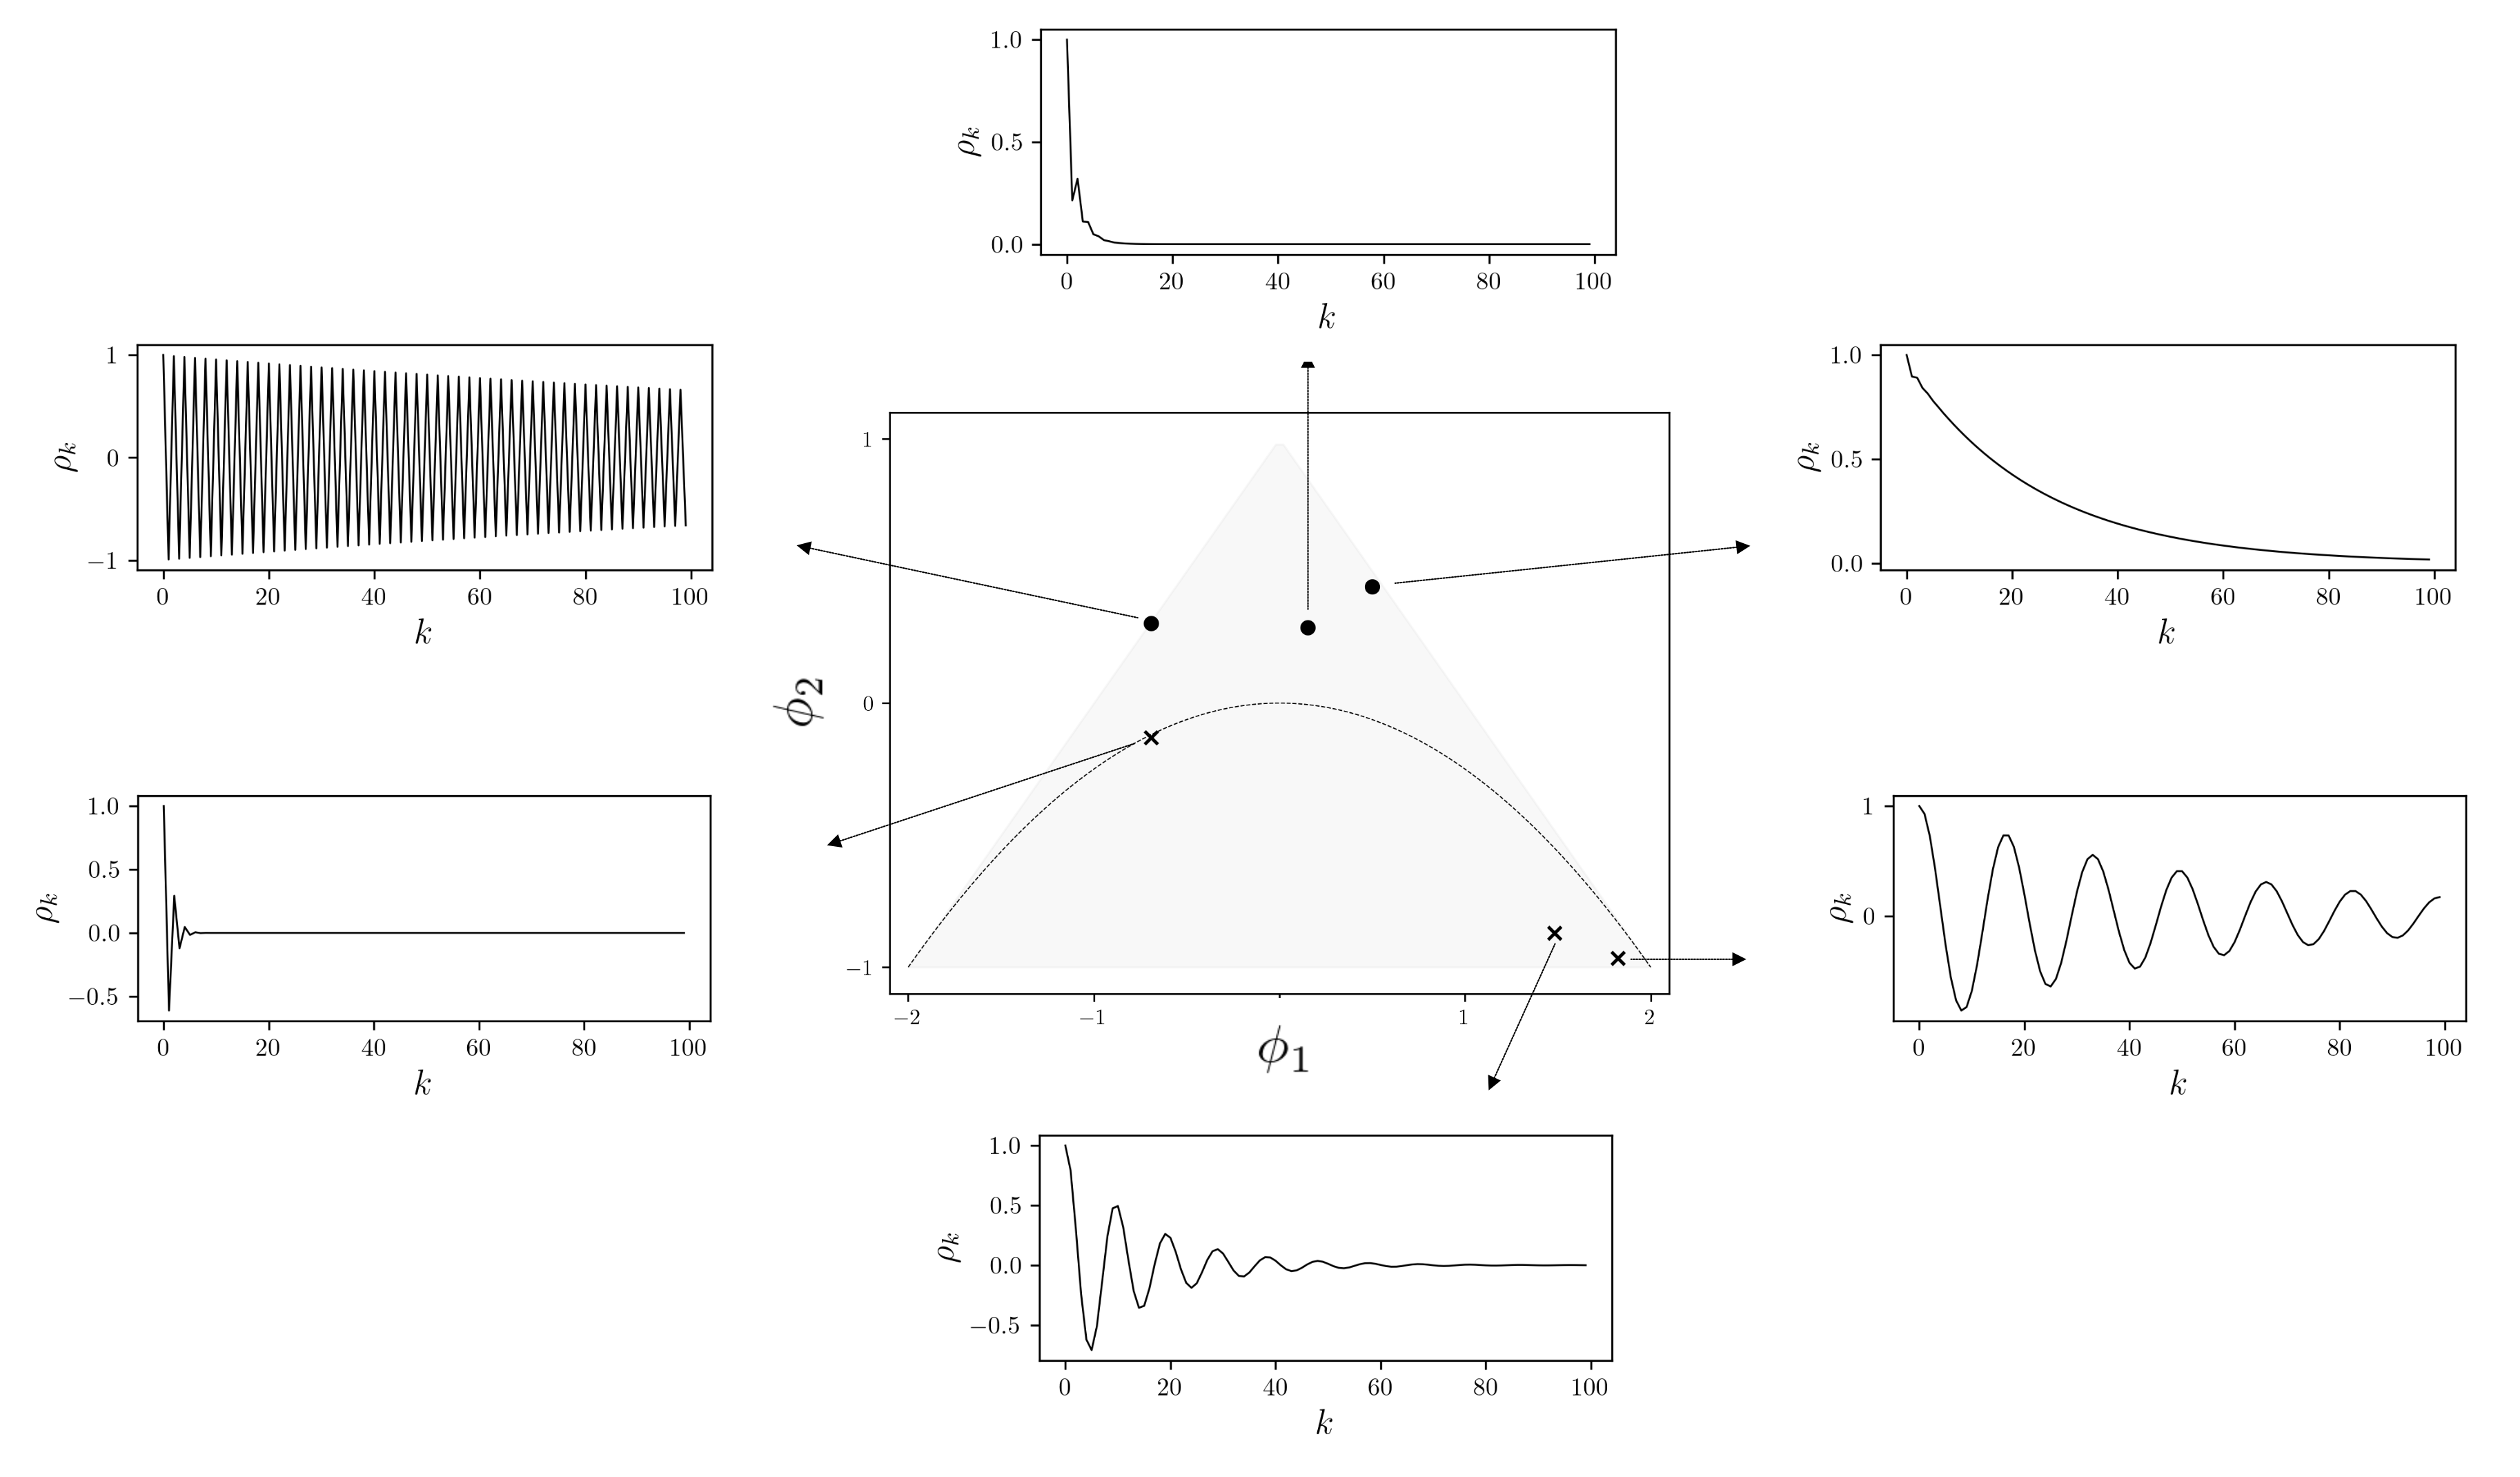
\includegraphics[width=0.99\textwidth]{latex/slides/ar2-stationary-triangle.png}}
\end{frame}

% slide %
\begin{frame}{AR-2 Simulation}
\footnotesize
\begin{itemize}
    \item \textbf{Setting}: $T = 4800$ timepoints, $N = 1000$ repeats.
    \item \textbf{AR process}: $x_t = \phi_1 x_{t-1} + \phi_2 x_{t-2} + e_t, \quad e_t \overset{iid}{\sim} \mathcal{N}(0, 1)$
    \item \textbf{Parameters}:\\
    $[\phi_1, \phi_2] \in \{\textcolor[HTML]{000000}{[0.1,0.1]}, \textcolor[HTML]{B66B7C}{[0.2,0.2]}, \textcolor[HTML]{8D9FCB}{[0.4,0.2]}, \textcolor[HTML]{66C2A6}{[0.5,0.2]}, \textcolor[HTML]{7D7D7D}{[0.7,0.2]}\}$\\
\end{itemize}
\vspace{0.25cm}
\centering
\visible{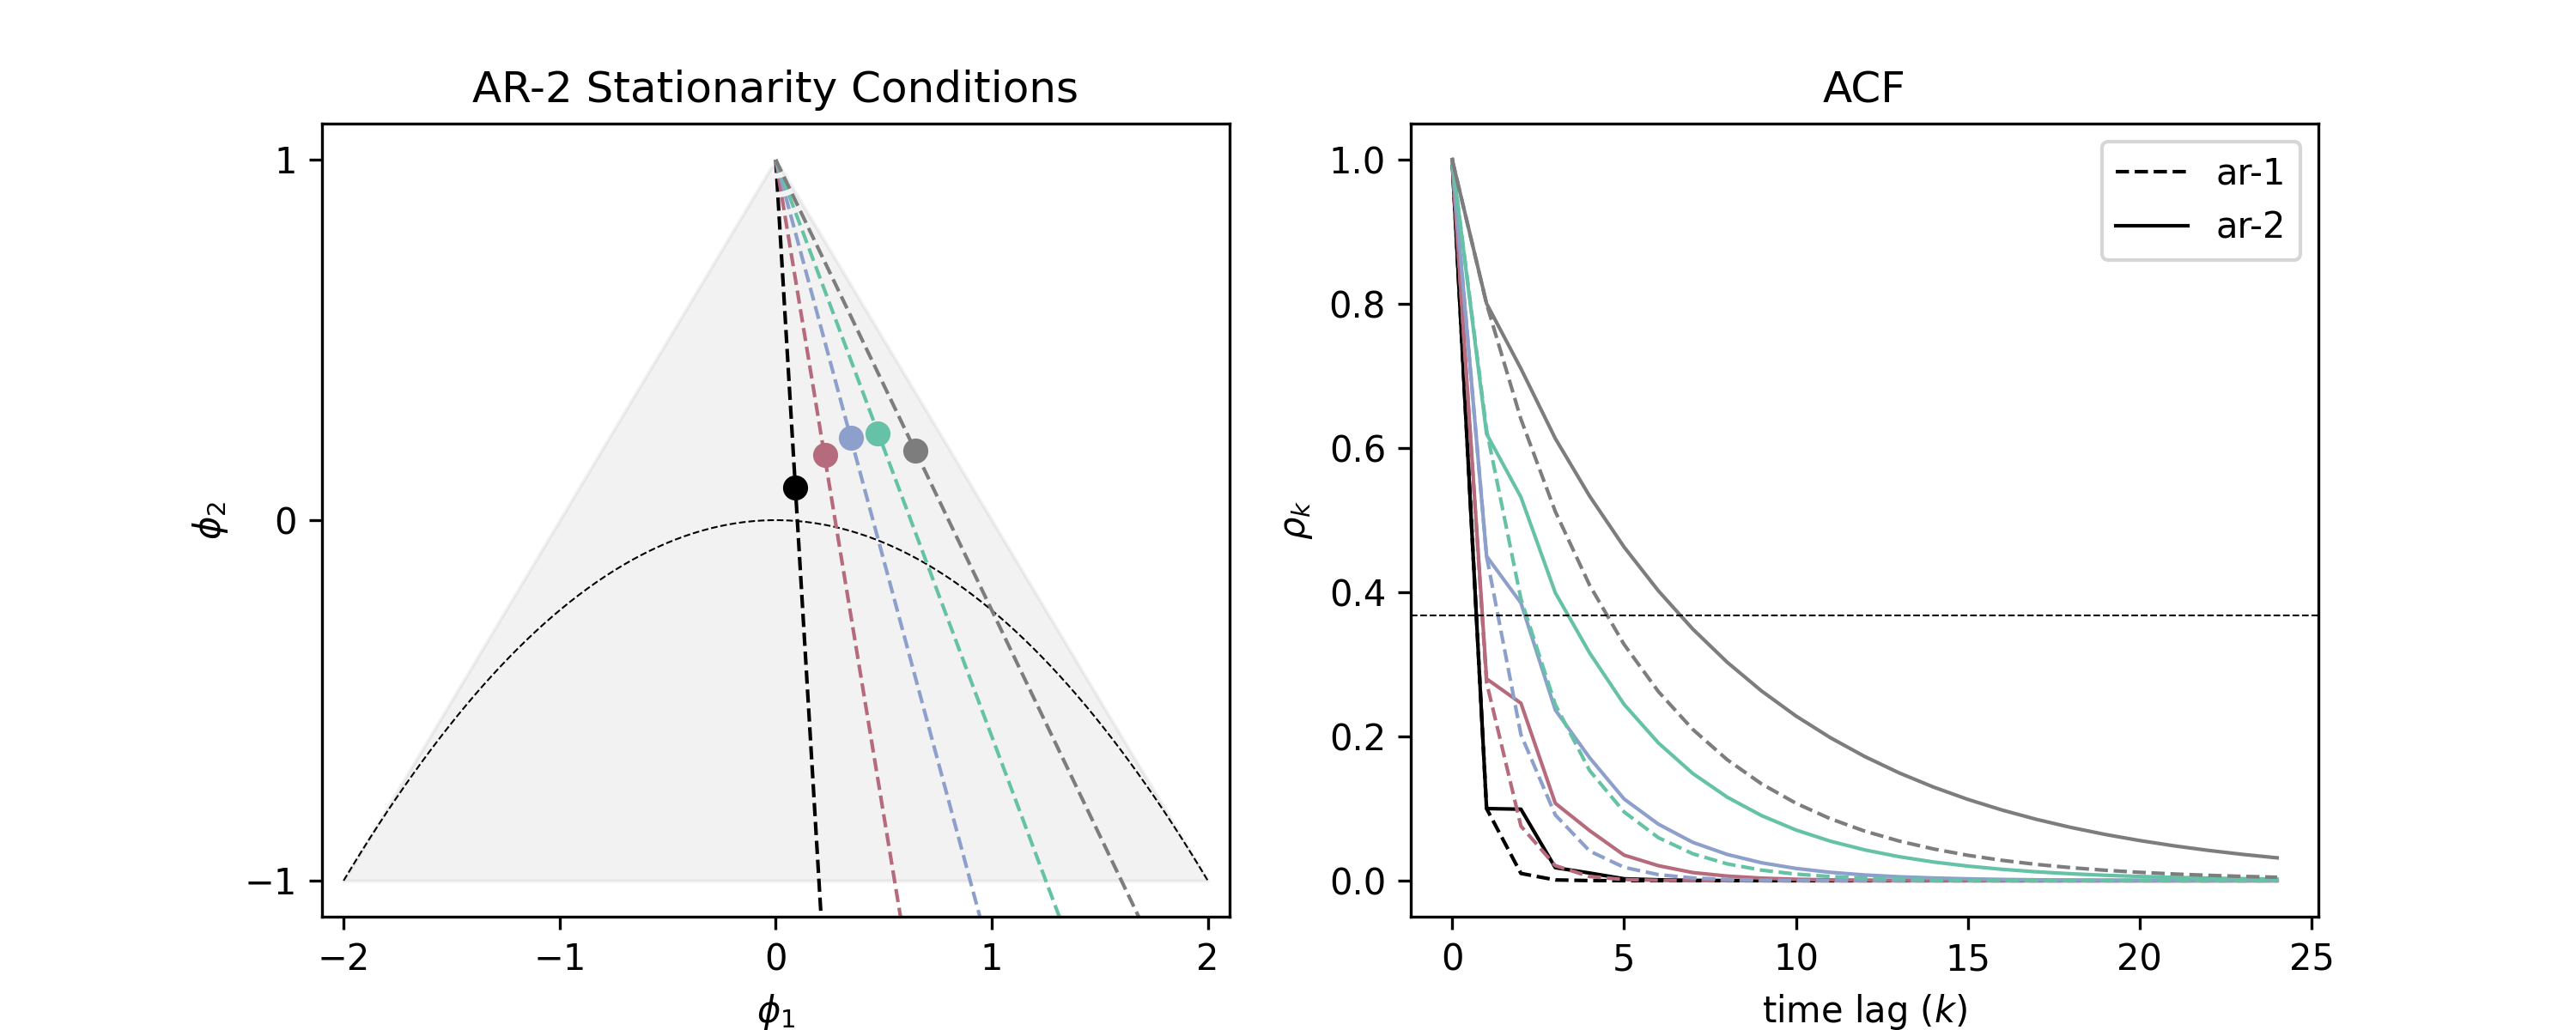
\includegraphics[width=0.9\textwidth]{latex/slides/simulations-ar2.png}}
\end{frame}

% slide %
\begin{frame}{AR-2 Results}
    \visible{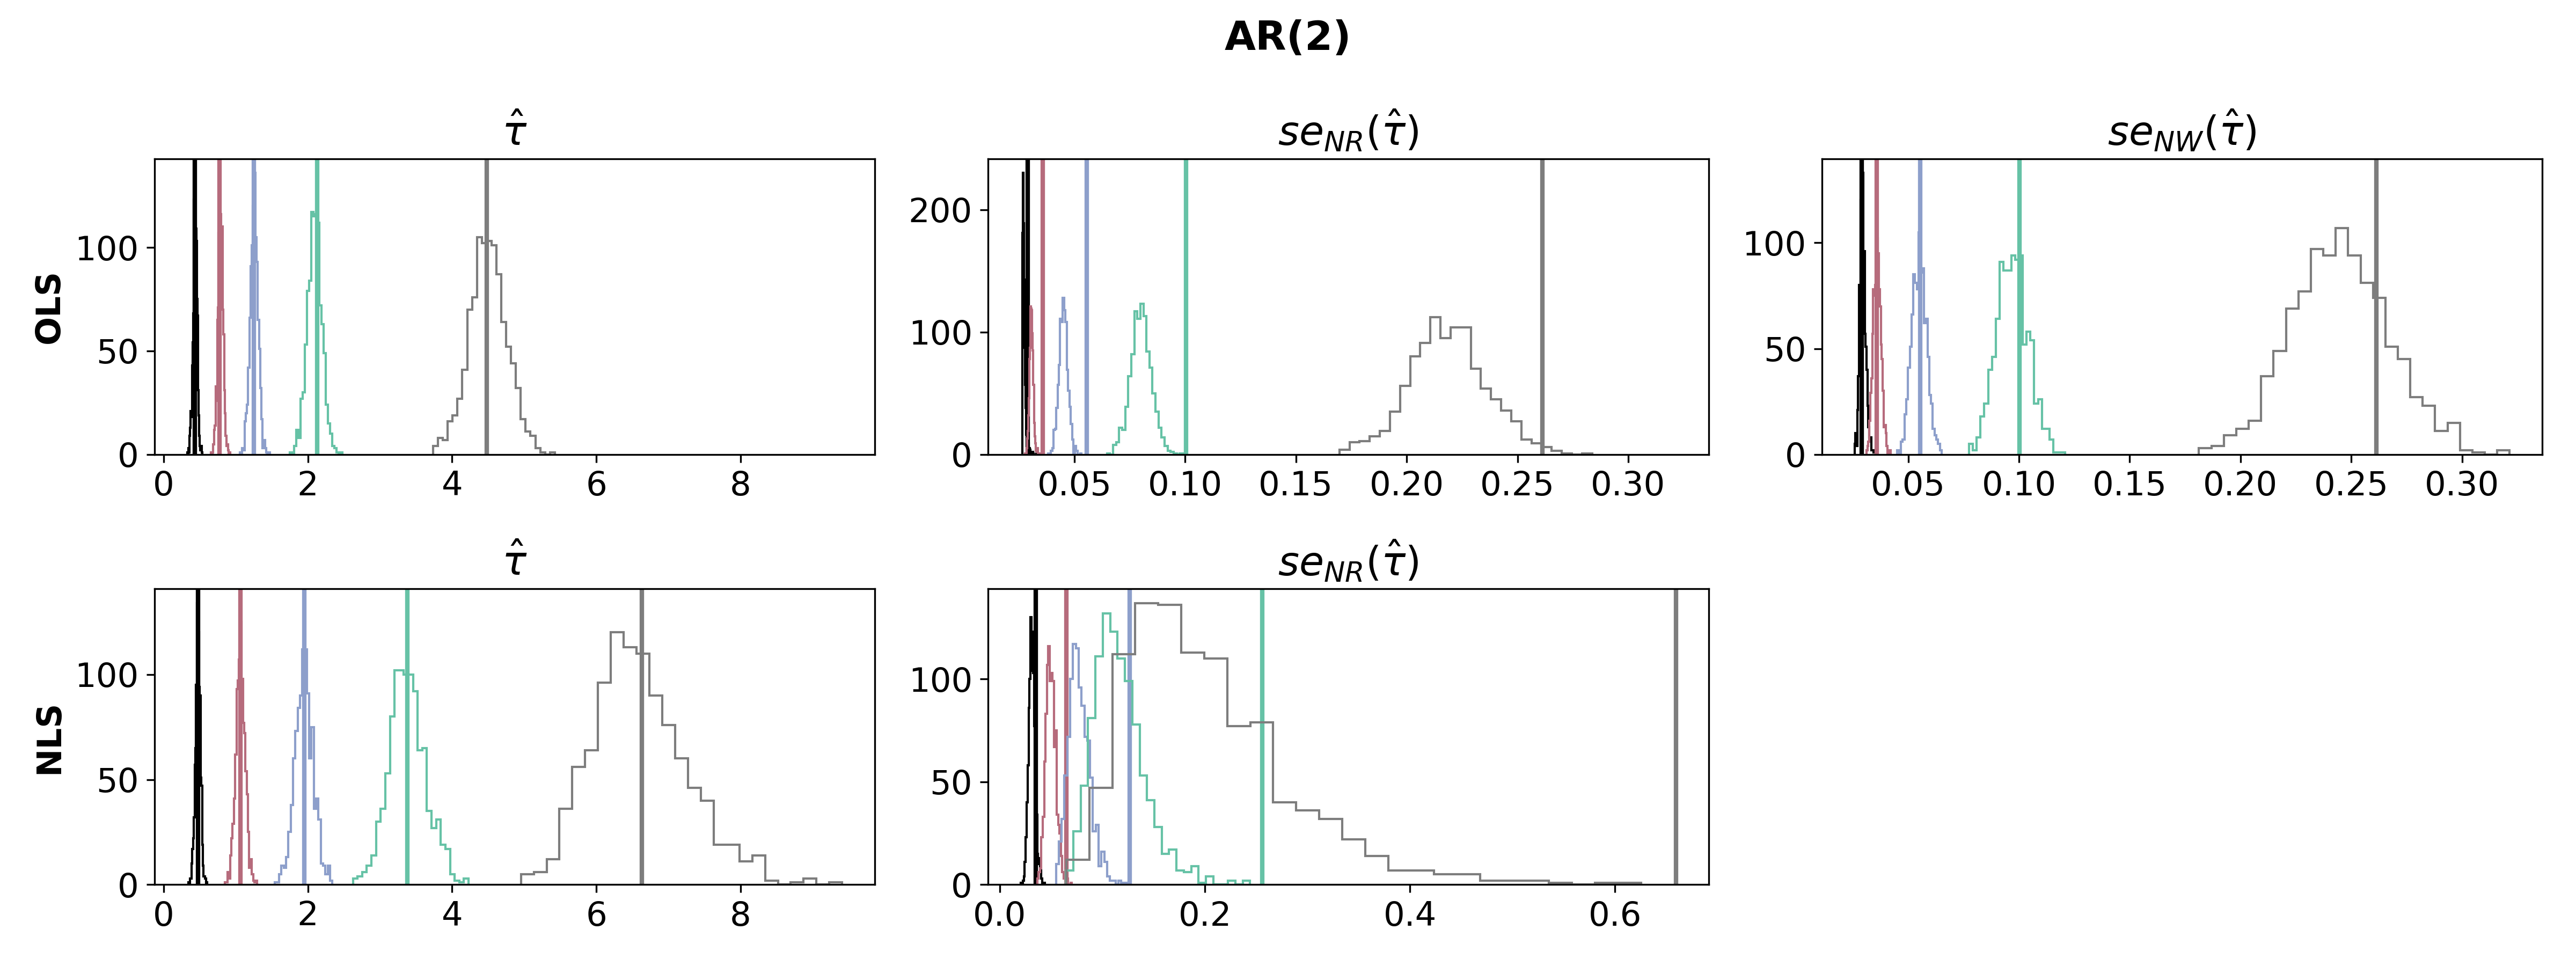
\includegraphics[width=1\textwidth]{latex/slides/sim-ar2.png}}
\end{frame}

% slide %
\subsection{HCP}
\begin{frame}{HCP Simulation}
\footnotesize
\begin{itemize}
    \item \textbf{Setting}: $T = 4800$ timepoints, $N = 1000$ repeats.
    \item \textbf{Parameters}:\\
    $\text{Brain Region} \quad \# \{\textcolor[HTML]{000000}{7}, \textcolor[HTML]{B66B7C}{12}, \textcolor[HTML]{8D9FCB}{126}, \textcolor[HTML]{66C2A6}{137}, \textcolor[HTML]{7D7D7D}{143}\}$\\
\end{itemize}

\centering
\visible{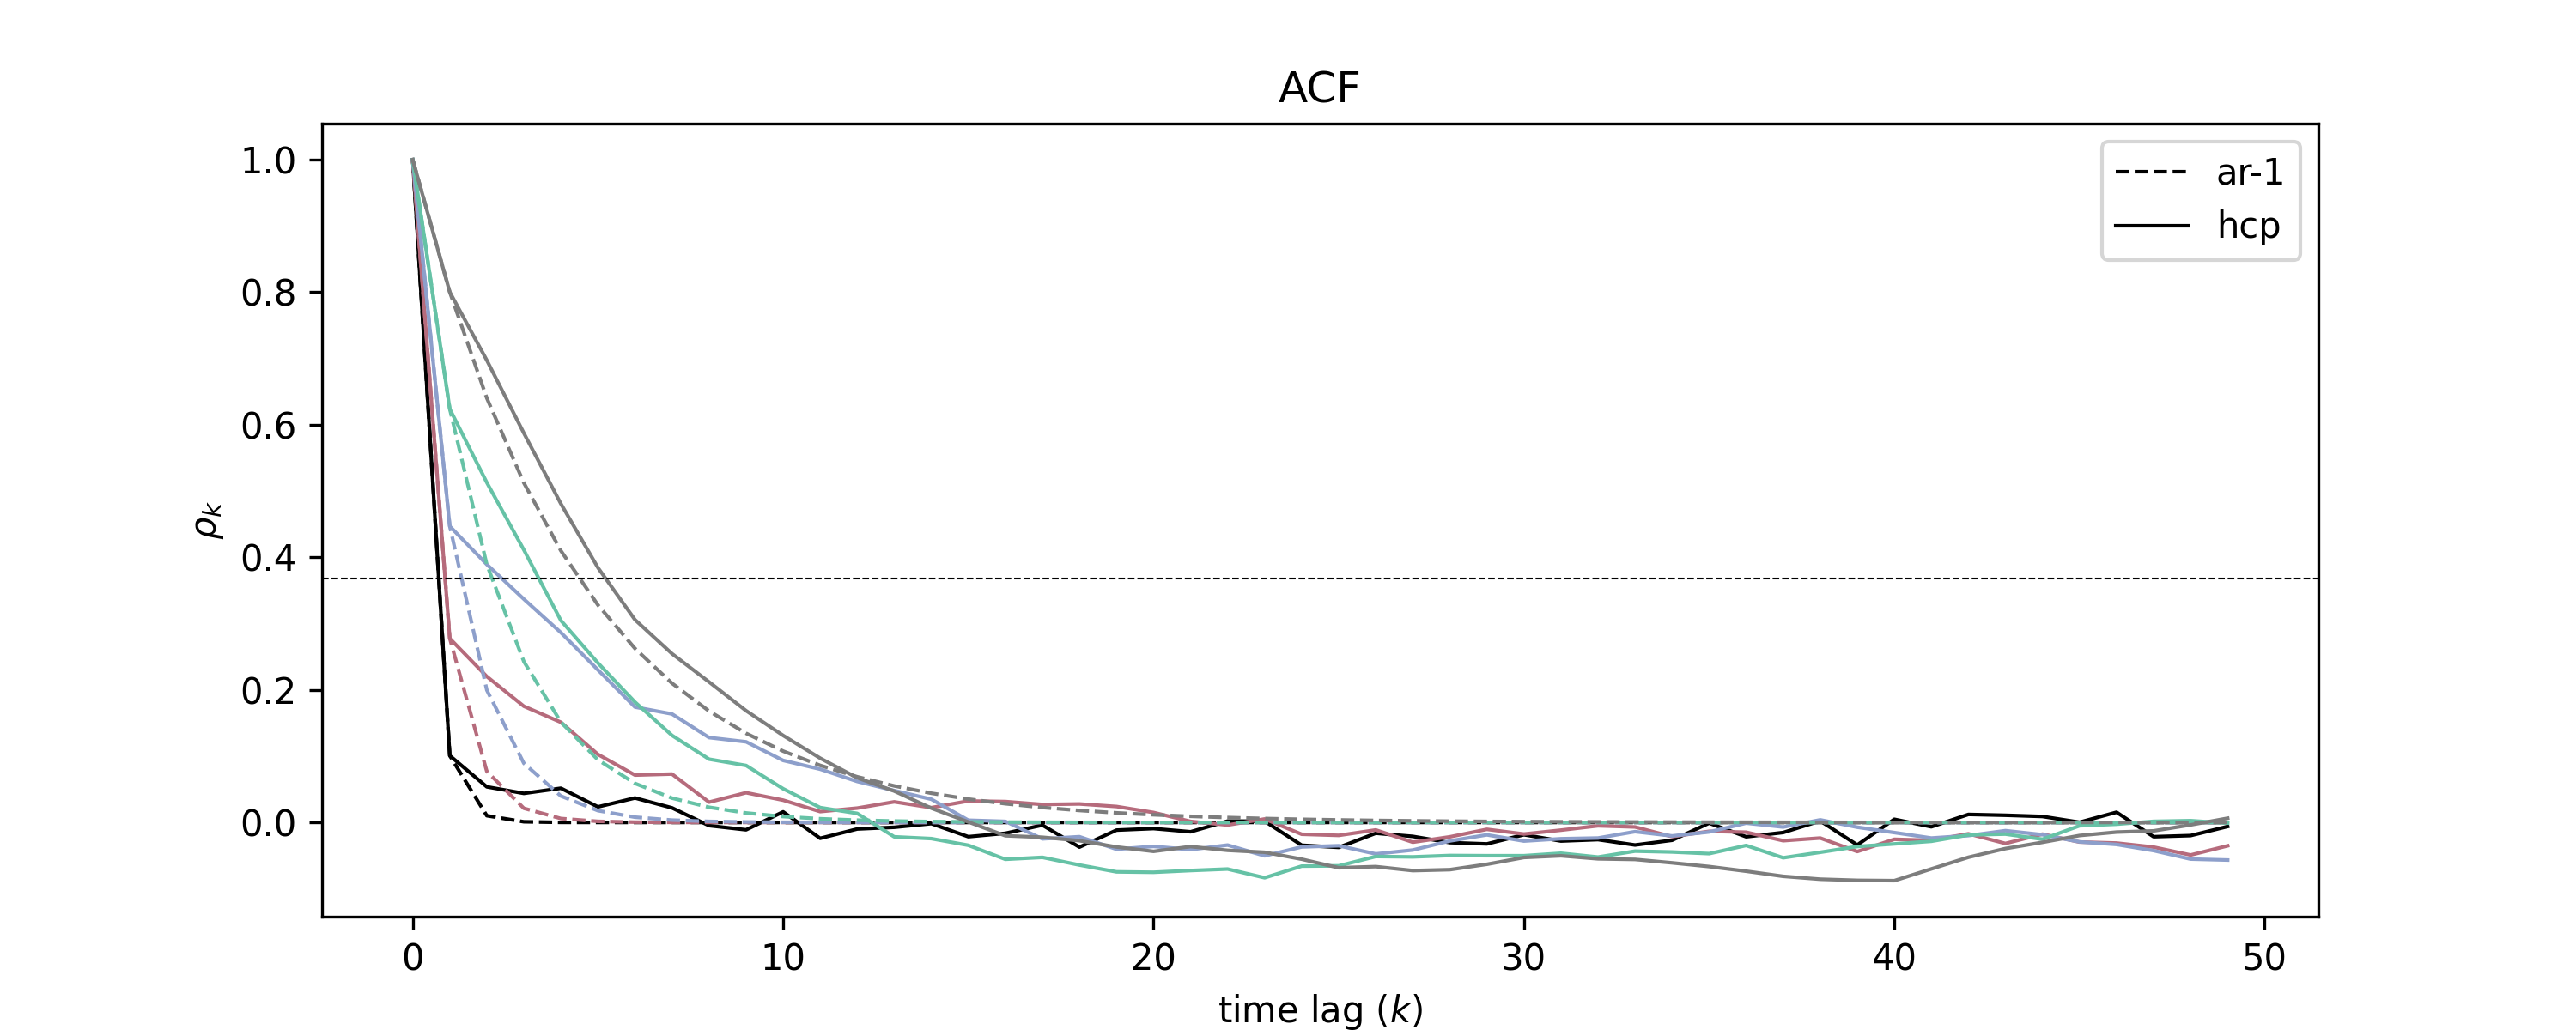
\includegraphics[width=0.6\textwidth]{latex/slides/simulations-hcp.png}}
\vspace{0.25cm}
\visible{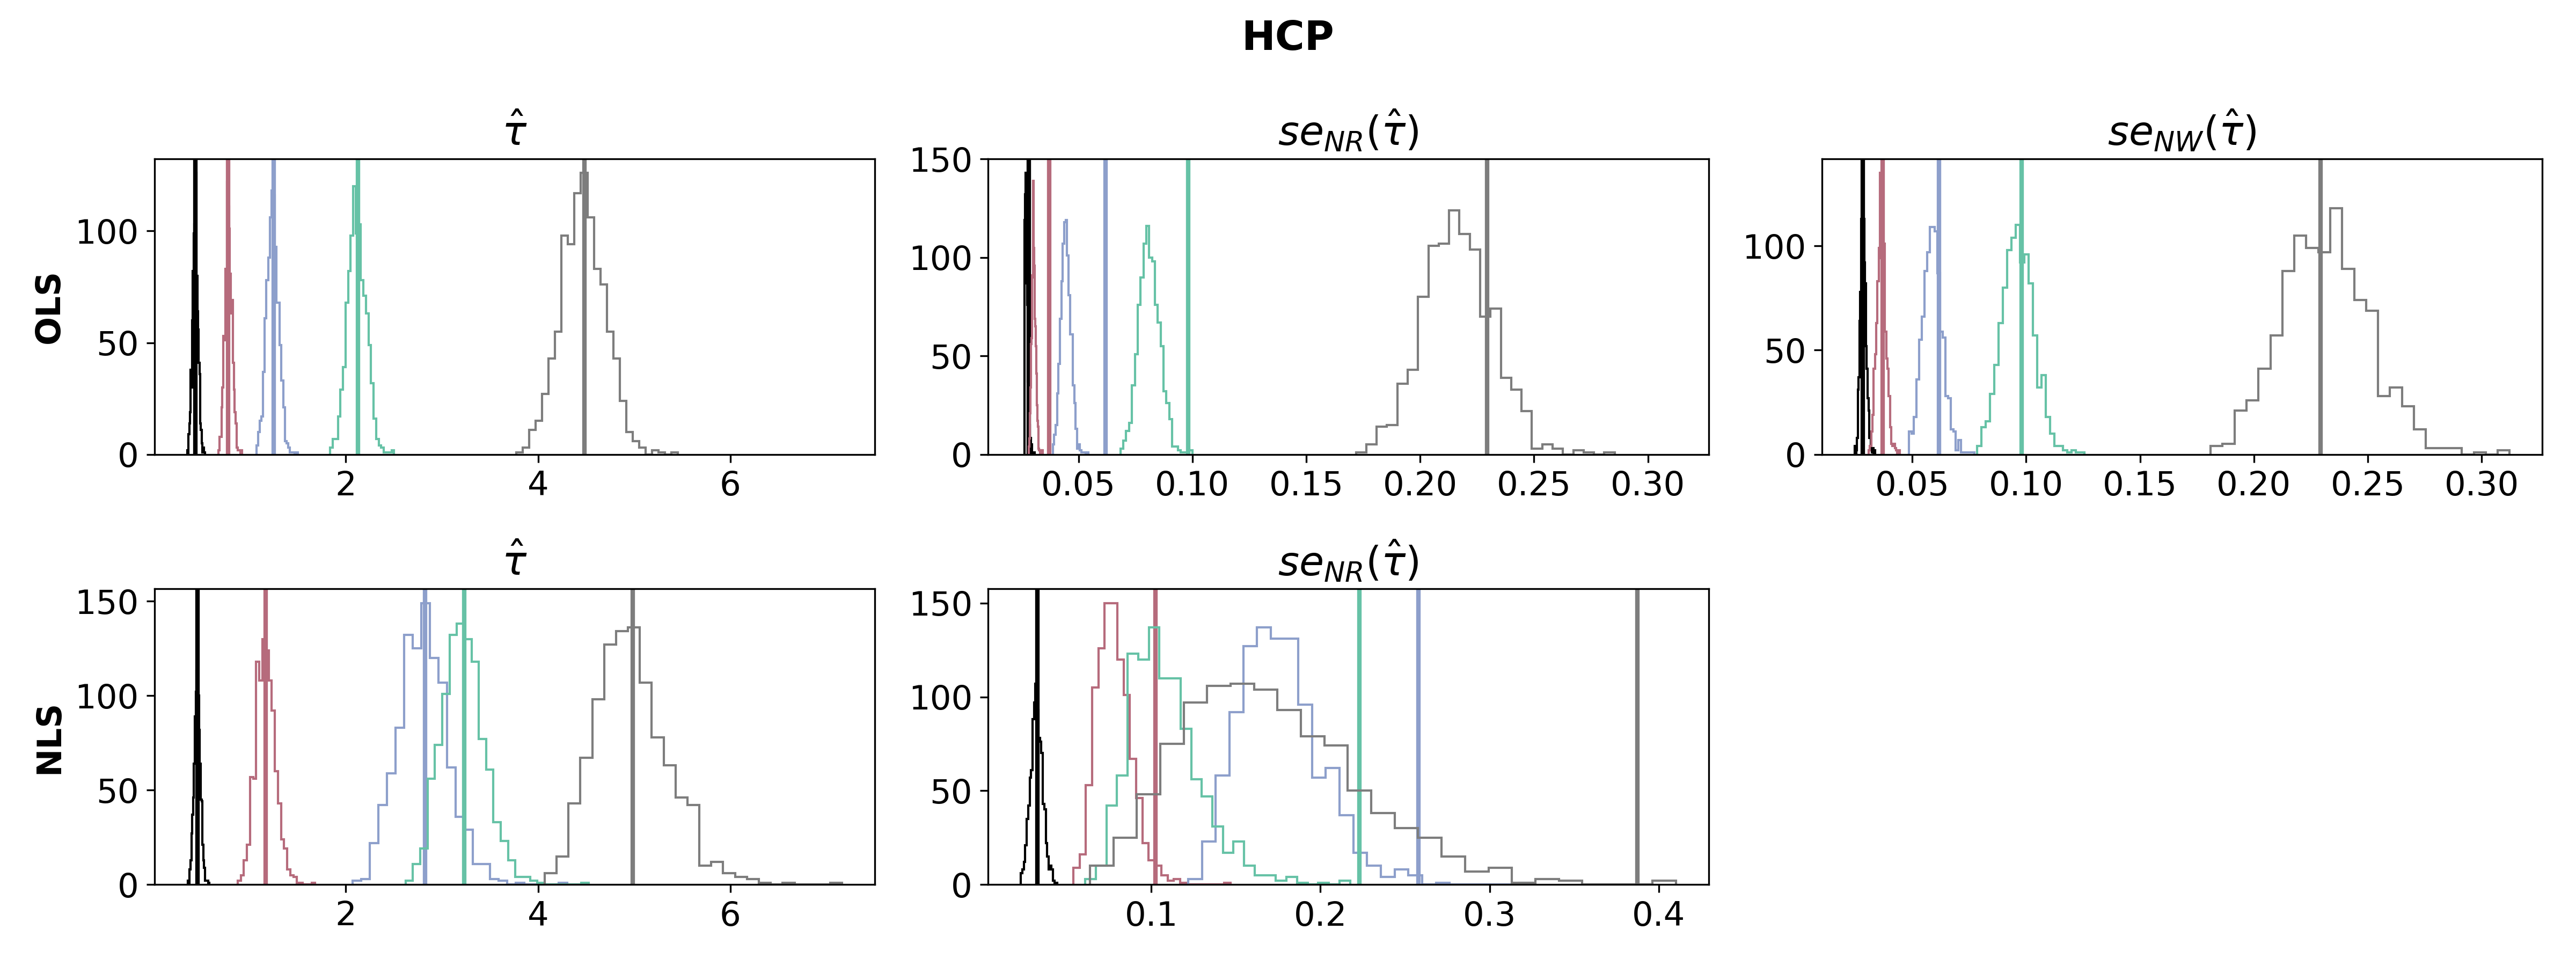
\includegraphics[width=1\textwidth]{latex/slides/sim-hcp.png}}
\end{frame}


\section{Applications}

% slide %
\subsection{Dataset Description}
\begin{frame}{Dataset Description}
    \centering
    \visible{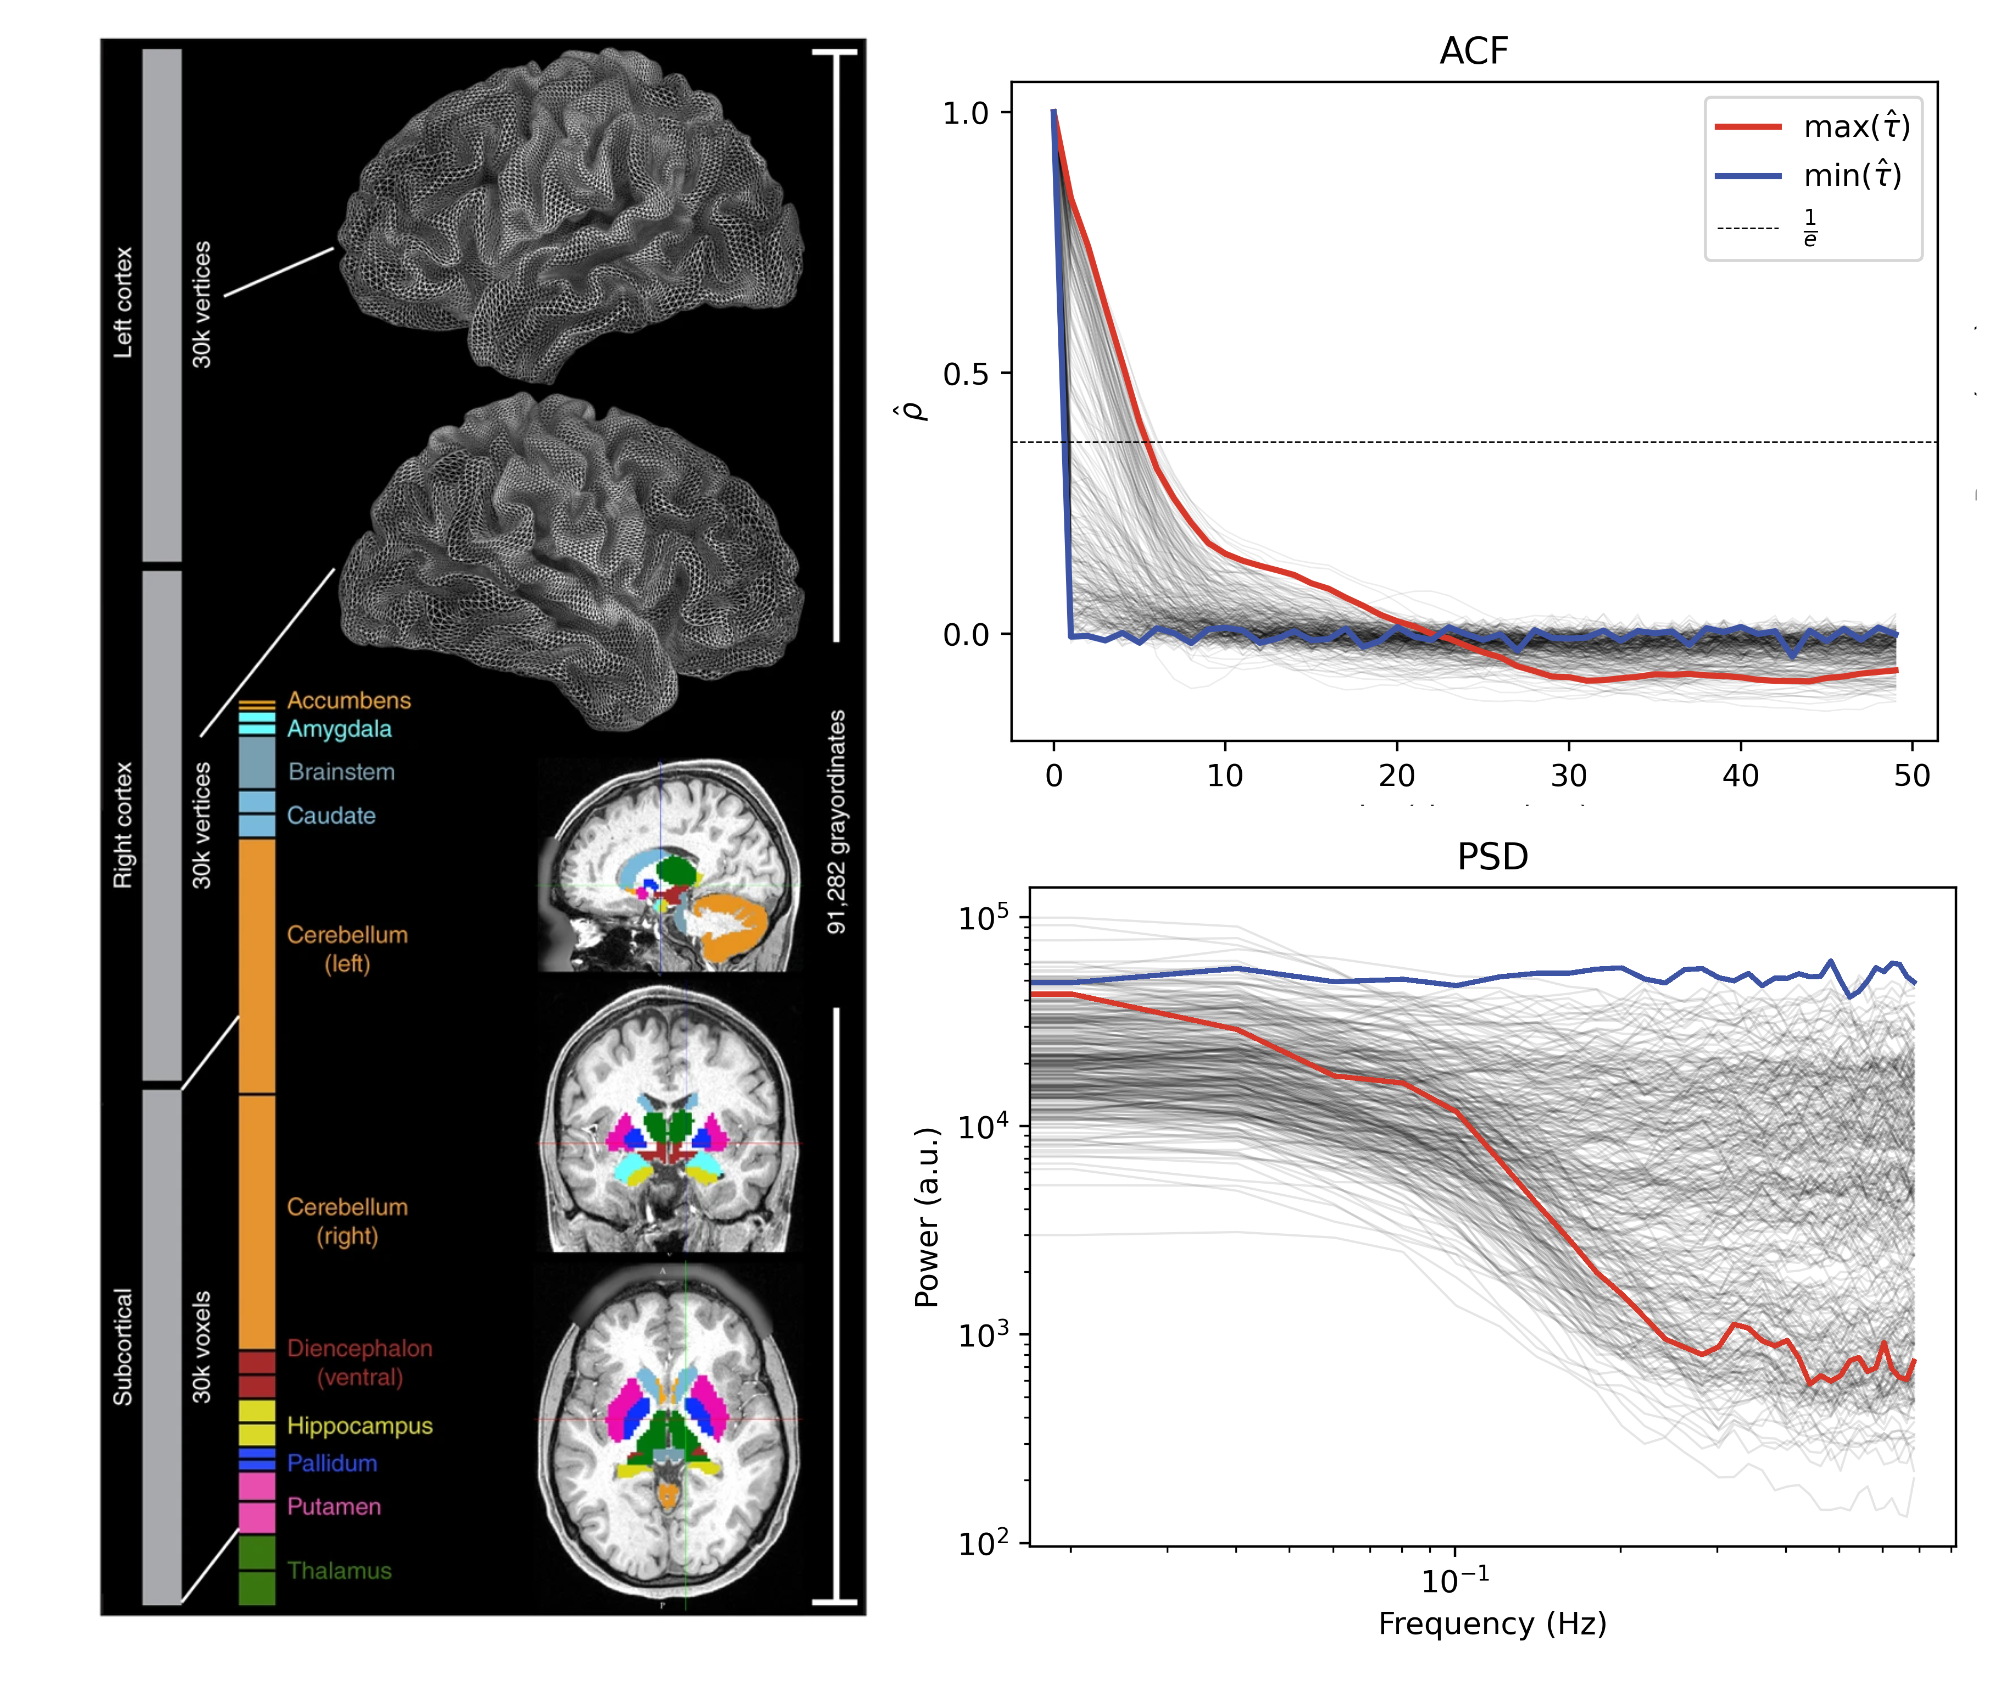
\includegraphics[width=0.85\textwidth]{latex/slides/dataset-description.png}}
    \scriptsize
    \begin{enumerate}
    \item Developing Methods: 10 subjects, 4800 timepoints, 300 regions
    \item \textbf{Estimating Maps:  184 subjects, 3600 timepoints, 91282 grayordinates}
    \end{enumerate}
\end{frame}

% slide %
\subsection{Timescale Maps}
\begin{frame}{Timescale Maps}
\scriptsize
$\hat \tau_{OLS}$
\visible{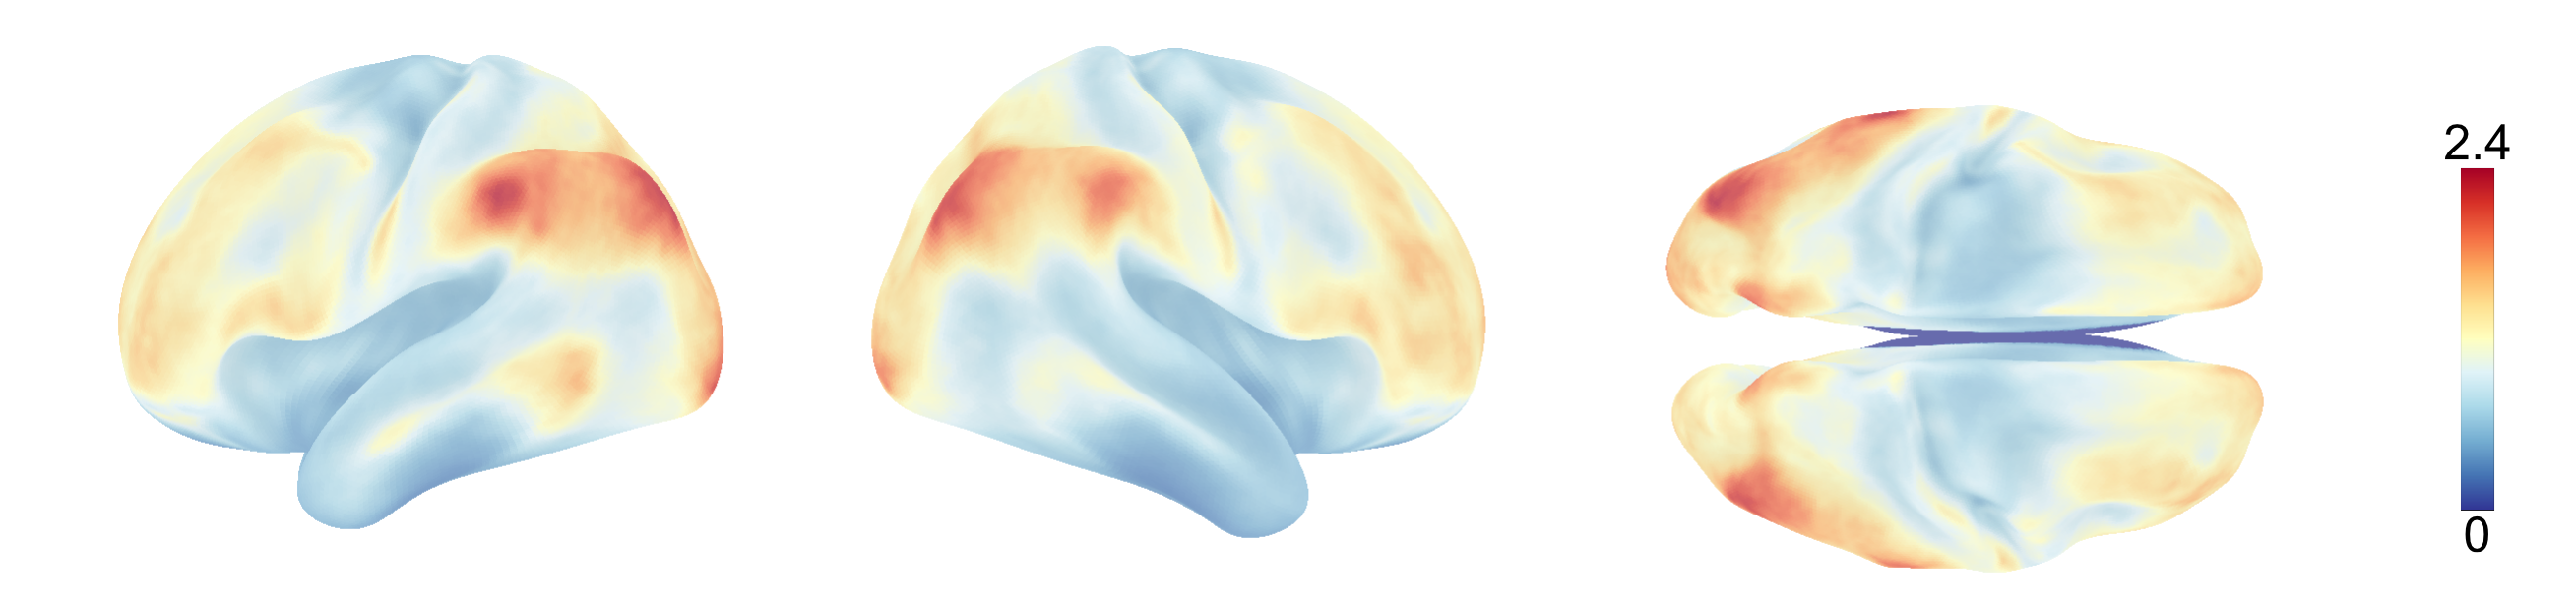
\includegraphics[width=1\textwidth]{latex/slides/tau_map.png}}
$\text{se}_{NW}(\hat \tau)$
\visible{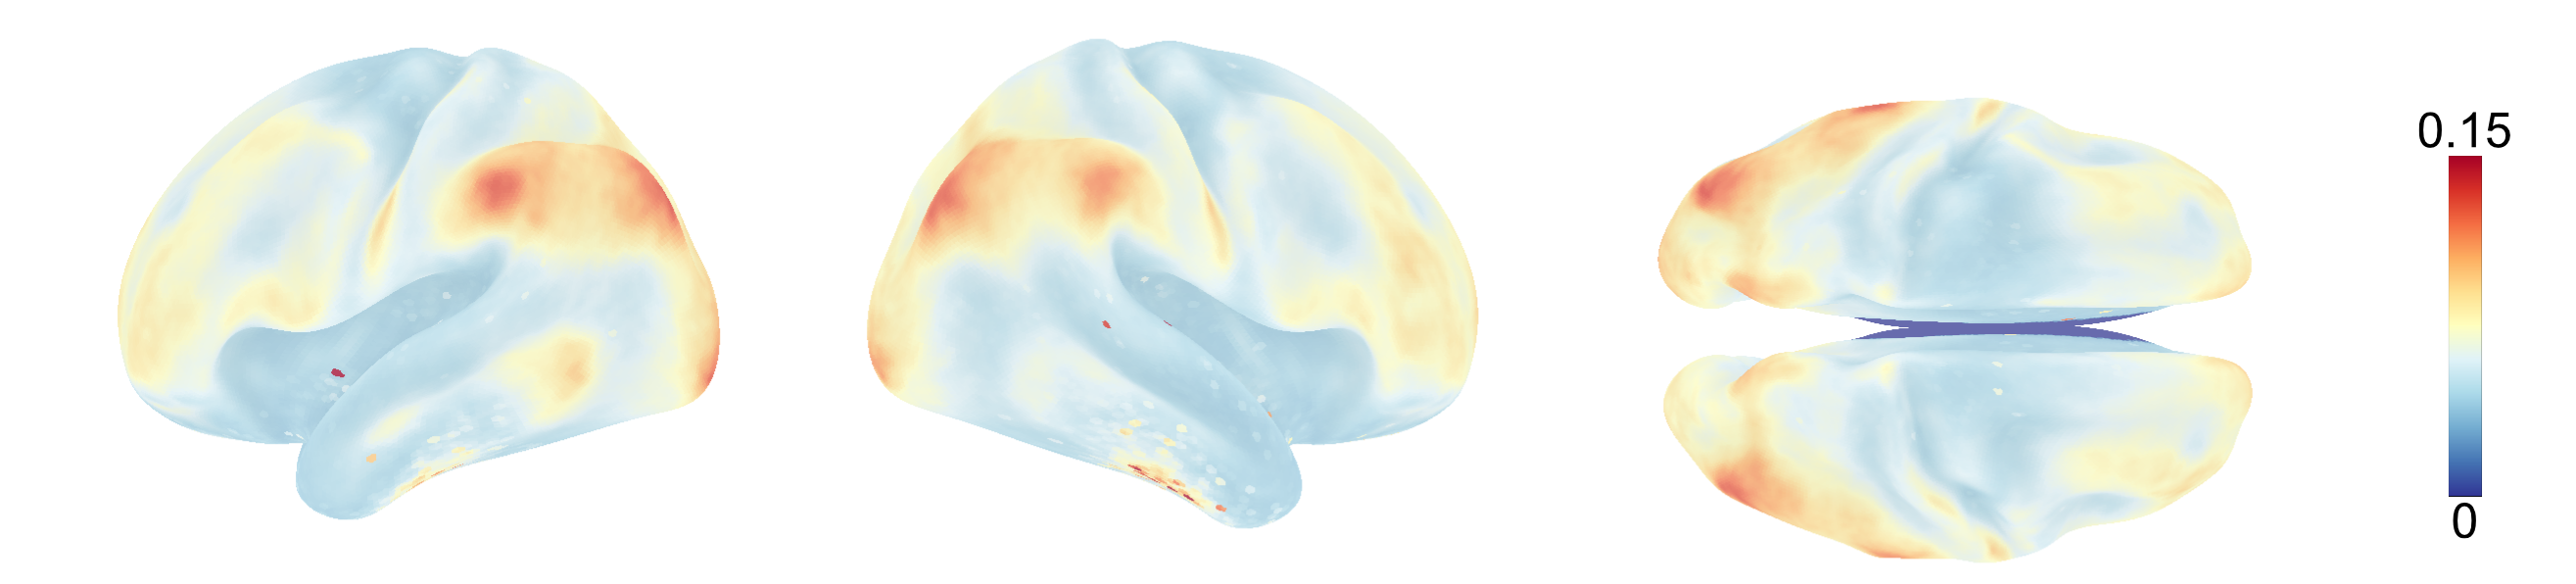
\includegraphics[width=1\textwidth]{latex/slides/se_map.png}}
$(\hat \tau_{OLS} - 1) / \text{se}_{NW}(\hat \tau)$
\visible{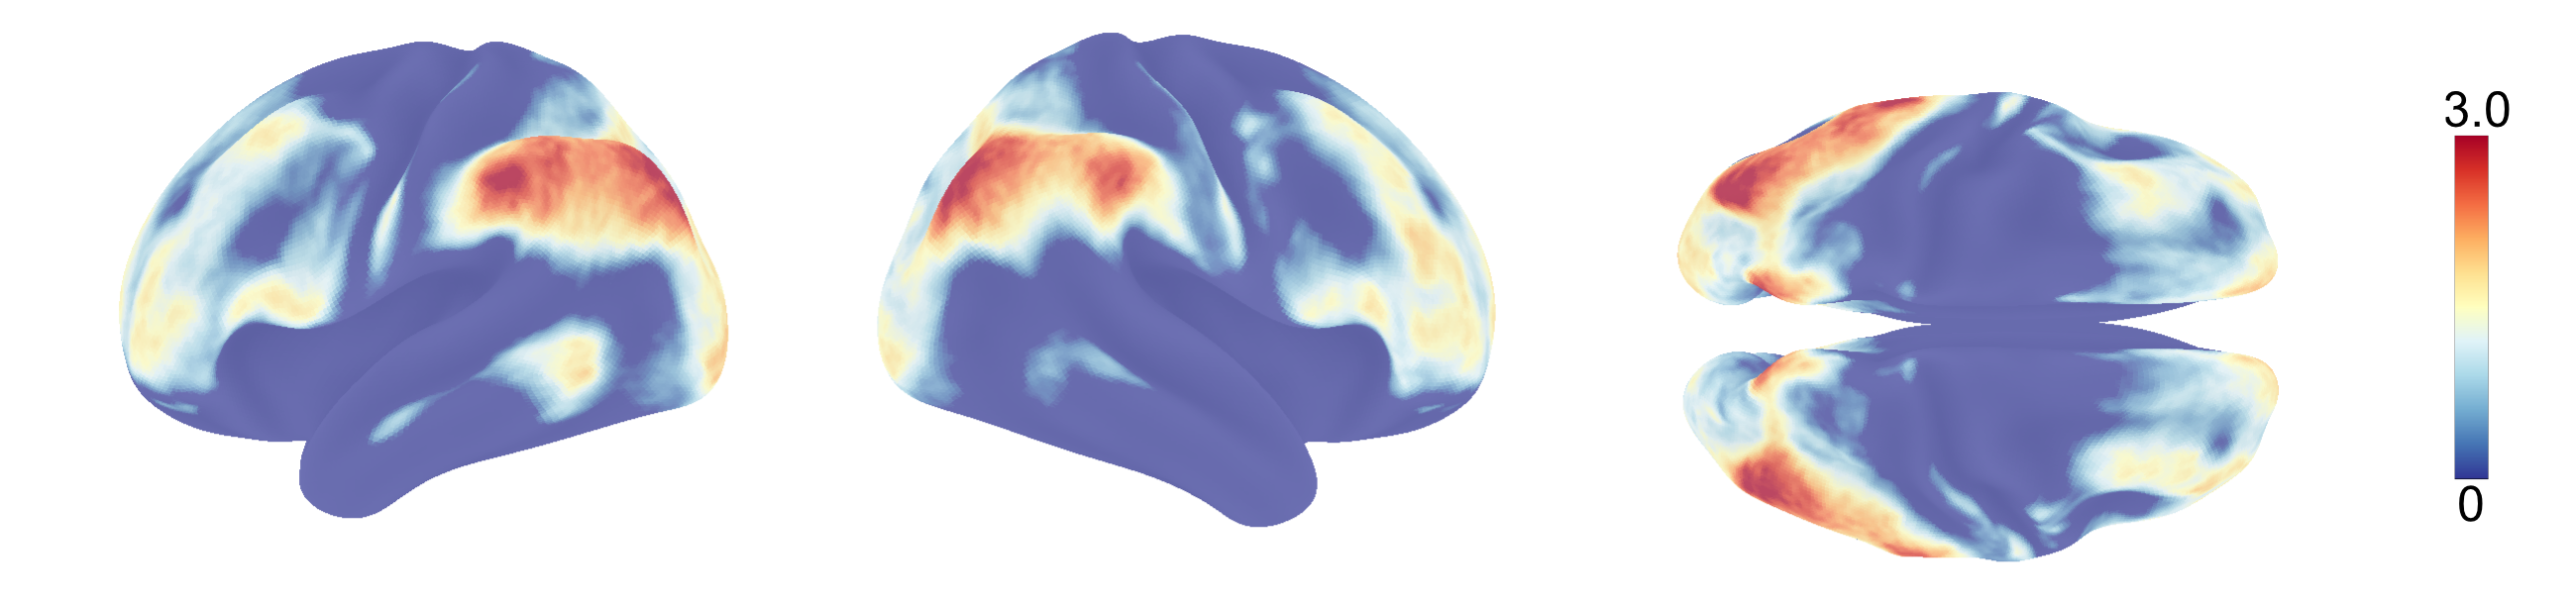
\includegraphics[width=1\textwidth]{latex/slides/tstat_map.png}}
\end{frame}

% slide %
\section{Conclusions}
\begin{frame}{Conclusions and Future Directions}
\textbf{Conclusions}:\\
\begin{itemize}
    \item Timescales (and their standard errors) can be accurately estimated, even if the models are misspecified
    \item Autoregressive models provide a computationally efficient alternative to exponential decay models
    \item The choice between the two depends on the trade off between dense sampling in time versus space
\end{itemize}

\textbf{Future Directions}:\\
\begin{itemize}
    \item Group-level models
    \item Nonstationary timeseries (autocorrelations that are time dependent)
    \item Multivariate settings (vector autoregession)
\end{itemize}
\end{frame}

% slide %
\section{References}
\begin{frame}{Acknowledgments}
Prof. Armin Schwartzman, Prof. Bradley Voytek, Dr. Samuel Davenport\\
\vspace{1cm}
\textbf{References}:\\
Papers:\\
\href{https://github.com/griegner/fmri-timescales/blob/master/latex/zotero.bib}{github.com/griegner/fmri-timescales/latex/zotero.bib}

\vspace{0.5cm}
Code:\\
\href{https://github.com/griegner/fmri-timescales}{github.com/griegner/fmri-timescales}
\end{frame}


% slide %
\section{Supplementary}
\subsection{Estimator Properties}

% slide %
\begin{frame}{Properties of OLS}
\vspace{0.25cm}
\footnotesize
\textbf{Consistency}: by the Ergodic and Continuous Mapping Theorems, the coefficients of an AR-1 model can be consistently estimated, as $T \to \infty$
\begin{align}
    \hat\phi = (\frac{1}{T} \sum_{t=2}^T x_{t-1}^2)^{-1} ( \frac{1}{T} \sum_{t=2}^T x_t x_{t-1}) &\underset{p}{\to} (\mathbb{E}[X_{t-1}^2])^{-1}(\mathbb{E}[X_t X_{t-1}]) = \phi
\end{align}

Similarly:
\begin{align}
    \hat \omega \underset{p}{\to} \omega
\end{align}

\onslide<2->
\textbf{Limiting variance}: as $T\to\infty$ we can approximate the asymptotic variance of $\phi$ and $\tau$ using a CLT for correlated observations (\cite{hansen_econometrics_2022}).
\begin{align}
\frac{\hat\phi - \phi}{\text{se}_{NW}(\hat\phi)} \underset{d}{\to} \mathcal{N}(0, 1)\\
\frac{\hat{\tau} - \tau}{\text{se}_{NW}(\hat{\phi}) \cdot \frac{d}{d\phi}(\hat\phi)} \underset{d}{\to} \mathcal{N}(0,1)
\end{align}
\end{frame}


\begin{frame}{Properties of NLS}
\footnotesize
\textbf{Consistency}: if the minimizer $\phi^k$ is unique, $S(\phi) > S(\phi^*)$ for all $\phi \ne \phi^*$, then as $K\to\infty$
\begin{align}
\hat \phi^* \underset{p}{\to} \phi^*
\end{align}

And under (??):\\
\begin{align}
\hat \omega \underset{p}{\to} \omega
\end{align}

\onslide<2->
\textbf{Limiting Variance}: as $K\to\infty$ we can approximate the asymptotic variance of $\phi$ and $\tau$ using a CLT for correlated observations (\cite{hansen_econometrics_2022}).

\begin{align}
\frac{\hat\phi^* - \phi^*}{\text{se}_{NW}(\hat\phi^*)} \underset{d}{\to} \mathcal{N}(0, 1)\\
\frac{\hat{\tau^*} - \tau^*}{\text{se}_{NW}(\hat{\phi^*}) \cdot \frac{d}{d\phi}g(\phi^*)} \underset{d}{\to} \mathcal{N}(0,1)
\end{align}
\end{frame}

\end{document}